% !TEX program = xelatex
% =============================================================================
% Block Round --- Plan de Aula (es-ES)
% Secuencia didactica de 5 sesiones para 2.o de Bachillerato (instituto publico
% espanol, modalidad Ciencias y Tecnologia / itinerario STEM), anclada en el
% universo Minecraft y en el marco normativo LOMLOE.
% Estilo grafico alineado con docs_math/Block_Round_Math_es-ES.pdf
% Compilacion: xelatex Plano_de_Aula_es-ES.tex  (ejecutar dos veces p/ TOC + refs)
% =============================================================================
\documentclass[12pt,a4paper]{scrartcl}

% ---------- Idioma y fuentes (identico a docs_math) -------------------------
\usepackage{fontspec}
\usepackage{polyglossia}
\setdefaultlanguage{spanish}
\PolyglossiaSetup{spanish}{indentfirst=false}
\setmainfont{Latin Modern Roman}[Scale=1.08]
\setsansfont{Latin Modern Sans}[Scale=1.08]
\setmonofont{Latin Modern Mono}[Scale=1.00]
\usepackage{unicode-math}
\setmathfont{Latin Modern Math}[Scale=1.08]

% ---------- Paquetes --------------------------------------------------------
\usepackage{amsmath}
\usepackage{mathtools}

\usepackage[a4paper,top=2.8cm,bottom=2.8cm,left=2.6cm,right=2.6cm,
            headheight=16pt]{geometry}
\usepackage{microtype}
\usepackage{xcolor}
\usepackage{booktabs}
\usepackage{array}
\usepackage{tabularx}
\usepackage{enumitem}
\usepackage{titlesec}
\usepackage{fancyhdr}
\usepackage{graphicx}
\usepackage{csquotes}
\usepackage{tcolorbox}
\tcbuselibrary{skins,breakable}
\usepackage{needspace}
\usepackage{caption}
\usepackage{subcaption}
\usepackage{float}

\raggedbottom

% ---------- Paleta cromatica Block Round ------------------------------------
\definecolor{accent}{HTML}{5B8E3F}      % verde-cesped Minecraft
\definecolor{accentdark}{HTML}{406A2A}
\definecolor{earth}{HTML}{825432}        % marron-tierra
\definecolor{ink}{HTML}{1F1F23}
\definecolor{muted}{HTML}{4E4E58}
\definecolor{bg}{HTML}{FBF6E9}
\definecolor{rule}{HTML}{D8D1BC}
\definecolor{linkc}{HTML}{2D5A1F}        % verde mas oscuro p/ enlaces

\usepackage[colorlinks=true,
            linkcolor=linkc,
            urlcolor=linkc,
            citecolor=linkc,
            breaklinks=true,
            bookmarks=true,bookmarksopen=true,
            pdftitle={Block Round --- Plan de Aula (es-ES)},
            pdfauthor={Vinicius Rodrigues de Souza}]{hyperref}
\usepackage{xurl}

\color{ink}

\widowpenalty=10000
\clubpenalty=10000

% ---------- Estilo de secciones ---------------------------------------------
\titleformat{\section}
  {\sffamily\Large\bfseries\color{accent}}{\thesection.}{0.6em}{}
\titleformat{\subsection}
  {\sffamily\large\bfseries\color{accent!85!ink}}{\thesubsection}{0.6em}{}
\titleformat{\subsubsection}
  {\sffamily\normalsize\bfseries\color{muted}}{\thesubsubsection}{0.5em}{}
\titlespacing*{\section}{0pt}{1.2\baselineskip}{0.6\baselineskip}
\titlespacing*{\subsection}{0pt}{0.8\baselineskip}{0.3\baselineskip}
\titlespacing*{\subsubsection}{0pt}{0.6\baselineskip}{0.2\baselineskip}

% ---------- Cabecera y pie de pagina ----------------------------------------
\pagestyle{fancy}
\fancyhf{}
\fancyhead[L]{\small\sffamily\bfseries\color{accent}BLOCK ROUND}
\fancyhead[R]{\small\sffamily\color{muted}Plan de Aula --- 2.\textordmasculine\ Bachillerato}
\fancyfoot[L]{\small\sffamily\color{muted}Block Round --- Material didactico}
\fancyfoot[R]{\small\sffamily\color{muted}Pagina \thepage}
\renewcommand{\headrulewidth}{0.4pt}
\renewcommand{\footrulewidth}{0.4pt}
\renewcommand{\headrule}{{\color{rule}\hrule height \headrulewidth}}
\renewcommand{\footrule}{{\color{rule}\vskip-\footrulewidth\hrule height \footrulewidth\vskip-\footrulewidth}}

% ---------- Cajas didacticas -------------------------------------------------
\newtcolorbox{formula}{
  colback=bg, colframe=rule, boxrule=0.4pt, arc=2pt,
  left=10pt,right=10pt,top=8pt,bottom=8pt,
  before skip=8pt, after skip=8pt,
  fontupper=\color{accentdark}, breakable,
  before={\par\needspace{4\baselineskip}}
}

\newtcolorbox{actividad}[1][Actividad]{
  enhanced, breakable,
  colback=bg, colframe=accent, boxrule=0.6pt, arc=4pt,
  left=12pt,right=12pt,top=10pt,bottom=10pt,
  before skip=12pt, after skip=12pt,
  before={\par\needspace{5\baselineskip}},
  attach boxed title to top left={xshift=10pt,yshift=-8pt},
  boxed title style={colback=accent,colframe=accent,boxrule=0pt,arc=2pt},
  coltitle=white, fonttitle=\sffamily\bfseries\small,
  title=#1
}

\newtcolorbox{nota}[1][Nota didactica]{
  enhanced, breakable,
  colback=bg!50!white, colframe=rule, boxrule=0.4pt, arc=2pt,
  left=10pt,right=10pt,top=8pt,bottom=8pt,
  before skip=8pt, after skip=8pt,
  before={\par\needspace{3\baselineskip}},
  attach boxed title to top left={xshift=10pt,yshift=-7pt},
  boxed title style={colback=muted,colframe=muted,boxrule=0pt,arc=2pt},
  coltitle=white, fonttitle=\sffamily\bfseries\footnotesize,
  title=#1
}

\newtcolorbox{competencia}[1][LOMLOE]{
  enhanced,
  breakable=false,
  colback=bg!70!white, colframe=accent!60!ink, boxrule=0.4pt, arc=2pt,
  left=10pt,right=10pt,top=6pt,bottom=6pt,
  before skip=6pt, after skip=6pt,
  before={\par\needspace{8\baselineskip}},
  attach boxed title to top left={xshift=10pt,yshift=-6pt},
  boxed title style={colback=accent!60!ink,colframe=accent!60!ink,boxrule=0pt,arc=2pt},
  coltitle=white, fonttitle=\sffamily\bfseries\footnotesize,
  title=#1
}

\newtcolorbox{minecraft}[1][Minecraft]{
  enhanced, breakable,
  colback=accent!7, colframe=earth!70!accent, boxrule=0.5pt, arc=3pt,
  left=10pt,right=10pt,top=8pt,bottom=8pt,
  before skip=10pt, after skip=10pt,
  before={\par\needspace{3\baselineskip}},
  attach boxed title to top left={xshift=10pt,yshift=-7pt},
  boxed title style={colback=earth,colframe=earth,boxrule=0pt,arc=2pt},
  coltitle=white, fonttitle=\sffamily\bfseries\footnotesize,
  title=#1
}

\setlength{\parskip}{0.75em}
\setlength{\parindent}{0pt}
\linespread{1.10}

\setlength{\textfloatsep}{14pt plus 2pt minus 2pt}
\setlength{\floatsep}{14pt plus 2pt minus 2pt}
\setlength{\intextsep}{14pt plus 2pt minus 2pt}

\captionsetup{font=small, labelfont={bf,color=accent}, textfont={color=muted}, justification=centering}
\captionsetup[sub]{font=footnotesize, labelfont={bf,color=accent!75!ink}, textfont={color=muted}}

\graphicspath{{img/}}

\newcommand{\code}[1]{\texttt{\small #1}}
\newcommand{\acc}[1]{\textcolor{accent}{\textbf{#1}}}
\newcommand{\cmd}[1]{\textcolor{earth}{\texttt{\small #1}}}
\newcommand{\tempo}[1]{\textnormal{\footnotesize\color{bg!90!white}\textsf{#1}}}

\begin{document}

% =============================================================================
% PORTADA
% =============================================================================
\begin{titlepage}
  \centering
  \vspace*{3.0cm}
  {\sffamily\bfseries\fontsize{56}{60}\selectfont \color{accent} Block Round\par}
  \vspace{0.7cm}
  {\sffamily\LARGE\color{muted} Plan de Aula\par}
  \vspace{0.25cm}
  {\sffamily\Large\color{muted} 2.\textordmasculine\ de Bachillerato\par}
  \vspace{1.0cm}
  {\color{rule}\rule{0.6\textwidth}{0.6pt}\par}
  \vspace{0.7cm}
  \begin{minipage}{0.84\textwidth}
    \centering\color{ink}\large
    Secuencia didactica de cinco sesiones para presentar el generador
    \emph{Block Round} a grupos de 2.\textordmasculine\ de Bachillerato
    (Matematicas II, itinerario STEM) en institutos publicos espanoles.
    Articula \emph{geometria analitica}, \emph{pensamiento computacional},
    \emph{competencia digital} y \emph{construccion en el videojuego
    Minecraft} en torno a un unico problema: como representar una curva
    continua sobre una malla finita de voxeles, y como traducir esa
    representacion en una estructura construible dentro del universo
    cultural mas popular entre adolescentes espanoles.
  \end{minipage}
  \vspace{0.7cm}\\
  {\color{rule}\rule{0.6\textwidth}{0.6pt}\par}
  \vspace{0.9cm}
  \begin{minipage}{0.78\textwidth}
    \centering
    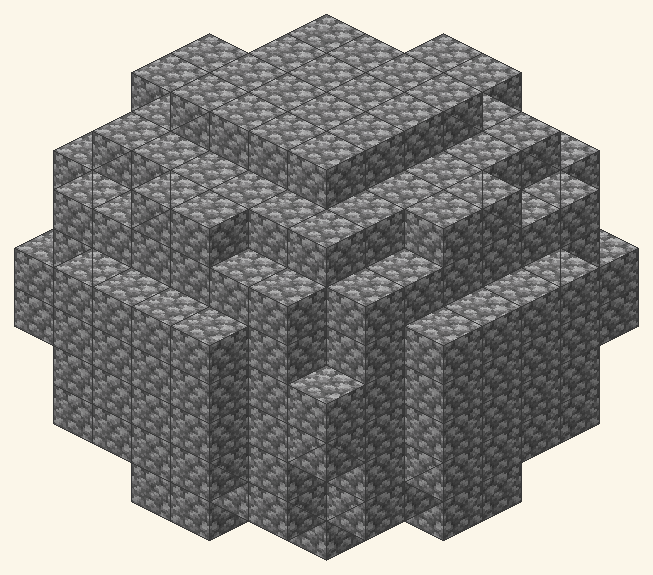
\includegraphics[width=0.55\linewidth]{fig10_3d_sphere_d12.png}\\[0.4em]
    {\sffamily\footnotesize\color{muted}Esfera de diametro 10 voxelizada por Block Round, renderizada con la textura \emph{cobblestone} (piedra de canto rodado) de Minecraft.}
  \end{minipage}
  \vspace{0.7cm}\\
  {\color{rule}\rule{0.6\textwidth}{0.6pt}\par}
  \vspace{0.9cm}
  \begin{minipage}{0.82\textwidth}
    \centering\sffamily\small\color{muted}
    \textbf{Areas integradas:} Matematicas $\cdot$ Lenguajes (Arte digital, Diseno) $\cdot$ Tecnologia e Informatica $\cdot$ Competencia Digital $\cdot$ Educacion para el ocio responsable \\[0.4em]
    \textbf{Marco normativo:} LOMLOE (Ley Organica 3/2020) $\cdot$ Real Decreto 217/2022 de Bachillerato $\cdot$ EvAU/EBAU Matematicas II $\cdot$ \hyperref[sec:ome]{OME-RSME} $\cdot$ Minecraft Education
  \end{minipage}
\end{titlepage}

% =============================================================================
\renewcommand{\contentsname}{\color{accent}Indice}
\tableofcontents
\thispagestyle{fancy}
\newpage

% =============================================================================
\section{Identificacion y contextualizacion}\label{sec:identificacion}

\begin{center}
\begin{tabular}{@{}p{0.32\textwidth}p{0.62\textwidth}@{}}
\toprule
\textbf{Materia} & Matematicas II (con fuerte articulacion interdisciplinar: Dibujo Artistico, Tecnologia e Ingenieria, Historia del Arte, Geografia). \\
\addlinespace[2pt]
\textbf{Etapa y curso} & Bachillerato --- 2.\textordmasculine\ curso, modalidad Ciencias y Tecnologia (y modalidad General con itinerario STEM). Adaptable a 1.\textordmasculine\ de Bachillerato (Matematicas I) y a Educacion de Personas Adultas (EPA/ESPA). \\
\addlinespace[2pt]
\textbf{Modalidades atendidas} & Bachillerato regular diurno y nocturno; Bachillerato a distancia (CIDEAD); EPA (Centros de Educacion de Personas Adultas); Bachillerato bilingue MEFP/British Council; modalidades de FP de grado superior con conexion STEM (Desarrollo de Aplicaciones, Animacion 3D, Sistemas Microinformaticos). \\
\addlinespace[2pt]
\textbf{Carga horaria} & 5 sesiones de 50 minutos (250 min en aula) + actividades de ampliacion opcionales. Variante de 2 sesiones dobles de 100 min descrita en §\ref{sec:adapt}. \\
\addlinespace[2pt]
\textbf{Recurso central} & Block Round --- aplicacion \emph{web} gratuita, sin registro, sin servidor, funciona \emph{offline} en el navegador (PWA). Conforme al RGPD y a la LOPDGDD: no recopila ni transmite datos personales. Funciona en \emph{smartphone} de gama baja --- no requiere Java, no requiere instalar Minecraft. \\
\addlinespace[2pt]
\textbf{Bloques de saberes basicos LOMLOE} & Bloque de Geometria (vectores, rectas, conicas, geometria analitica en el espacio) $\cdot$ Bloque de Analisis (volumenes y areas via integral) $\cdot$ Pensamiento Computacional como saber transversal $\cdot$ Competencia Digital (Marco DigComp 2.2). \\
\addlinespace[2pt]
\textbf{Itinerarios y conexiones} & Modalidad Ciencias y Tecnologia (principal) $\cdot$ Conexiones con Dibujo Tecnico II (geometria descriptiva), Tecnologia e Ingenieria, Fundamentos del Arte II. Itinerario STEM destacado en los curriculos autonomicos. \\
\addlinespace[2pt]
\textbf{Articulaciones} & \hyperref[sec:ome]{OME} (Olimpiada Matematica Espanola --- RSME) $\cdot$ OIE (Olimpiada Informatica Espanola --- SCIE) $\cdot$ Estalmat (Estimulo del Talento Matematico) $\cdot$ FECYT (Feria de la Ciencia) $\cdot$ Code Week EU $\cdot$ Minecraft Education Edition. \\
\addlinespace[2pt]
\textbf{Conocimientos previos del alumnado} & Sistema de coordenadas cartesianas; ecuacion de la circunferencia (1.\textordmasculine\ Bachillerato); areas y volumenes de cuerpos elementales; nocion de funcion; proporcion y porcentaje; operaciones con vectores en el plano. Familiaridad con \emph{Minecraft} (recomendable pero no obligatoria; el software \emph{Block Round} la suple). \\
\addlinespace[2pt]
\textbf{Preparacion del profesorado} & 20 minutos de exploracion previa de Block Round; lectura de \texttt{docs\_math/Block\_Round\_Math\_es-ES.pdf} (documento tecnico en espanol); opcionalmente, contacto superficial con los comandos \cmd{/fill}, \cmd{/clone} y \cmd{//sphere} de Minecraft Java Edition. \\
\bottomrule
\end{tabular}
\end{center}

\begin{nota}[Diversidad del sistema educativo espanol]
Esta secuencia se ha pensado para el contexto plural del Bachillerato publico espanol: el instituto urbano de Madrid, Barcelona, Sevilla, Valencia, Bilbao o Zaragoza; el instituto de cabecera de comarca; el Centro Integrado de Formacion Profesional (CIFP); el centro rural de la \enquote{Espana vaciada} (Teruel, Soria, Cuenca); los centros con alta proporcion de alumnado gitano o de migracion reciente; la EPA del turno nocturno; los centros bilingues BIE; los Bachilleratos Internacionales en centros publicos. Cada uno de estos contextos requiere ajustes especificos, recogidos en §\ref{sec:adapt}. Block Round se ha elegido porque \emph{atiende a todos ellos}: funciona en \emph{smartphone} economico, no necesita internet permanente despues de la primera carga (PWA), no exige registro ni datos personales --- condicion exigida por el RGPD (Reglamento UE 2016/679) y por la LOPDGDD (Ley Organica 3/2018).
\end{nota}

\begin{minecraft}[Por que anclar la secuencia en Minecraft]
Minecraft es el videojuego mas vendido de la historia (mas de 300 millones de copias). En Espana es referencia cultural transversal entre adolescentes de todas las comunidades autonomas y de todas las clases sociales, atravesando barreras de renta que otros videojuegos no consiguen (la version \emph{Bedrock} para movil cuesta menos de 8 euros, y existe \emph{Minecraft Education Edition} gratuita para centros via Microsoft 365 Educacion A1/A3, ya implantada en Comunidad de Madrid, Catalunya, Andalucia y otras). Los youtubers y streamers hispanohablantes mas vistos del mundo (Vegetta777, Willyrex, Rubius, AuronPlay, Mikecrack, TheGrefg) tienen a Minecraft como contenido central; series colaborativas como \emph{KarmaLand}, \emph{Egoland} y \emph{MinaCraft} han marcado a una generacion. \emph{Tomar Minecraft como mote no es una moda: es reconocer donde la juventud espanola ya vive y ya hace geometria.}
\end{minecraft}

% =============================================================================
\section{Justificacion pedagogica}\label{sec:justificativa}

La eleccion de Block Round como artefacto didactico para 2.\textordmasculine\ de Bachillerato responde a una demanda \acc{quintuple} de la educacion espanola contemporanea: integrar matematica formal y competencia digital (Marco DigComp 2.2 de la UE, incorporado por la LOMLOE); contextualizar el conocimiento abstracto en practicas \emph{significativas} para el alumnado; preparar para items de Geometria Analitica del Espacio y Calculo Integral recurrentes en la EvAU/EBAU de Matematicas II; dialogar con la LOMLOE (Ley Organica 3/2020) y con el Real Decreto 217/2022 de 29 de marzo, que regula las ensenanzas minimas de Bachillerato; y movilizar el universo cultural del videojuego \emph{Minecraft} como puente motivacional sin perder rigor matematico.

El \emph{voxel art} ocupa un lugar central en el imaginario juvenil espanol contemporaneo. \emph{Minecraft} --- juego nacido en 2009, comprado por Microsoft en 2014 por 2\,500 millones de dolares, hoy presente en centros educativos via \emph{Minecraft Education Edition} --- es la referencia cultural mas transversal entre adolescentes espanoles. Tomar la construccion en voxeles como punto de partida transforma una tradicion \emph{ludica} familiar en \emph{problema matematico genuino}: describir, en una rejilla discreta de bloques $1\times1\times1$, formas analiticamente definidas sobre $\mathbb{R}^3$. El alumno que construye a diario cubos, torres, granjas redondas y cupulas en el servidor de la comunidad descubre que aquello que ya hace por intuicion tiene nombre formal: \emph{voxelizacion}, \emph{rasterizacion discreta}, \emph{ecuacion implicita del elipsoide}.

Este movimiento didactico dialoga con cinco tradiciones de la pedagogia que han marcado al profesorado espanol:

\begin{itemize}[leftmargin=1.3em,itemsep=0.2em,topsep=0.3em]
  \item \acc{Francisco Giner de los Rios} (Institucion Libre de Ensenanza, 1876). El principio gineriano de partir del contacto del alumno con la realidad concreta --- y no de la abstraccion academica --- aproxima la secuencia a la nocion ginerista de \emph{aprendizaje activo}. El hecho de que el alumno \emph{ya sepa} construir esferas en Minecraft (aunque de forma intuitiva) lo situa como sujeto activo, no como recipiente pasivo. La ILE inspiro varias generaciones de profesorado renovador y sigue siendo referencia obligada en los Master de Profesorado de Secundaria.

  \item \acc{Lorenzo Milani} (\emph{Carta a una maestra}, 1967; obra traducida y difundida en Espana en los anos 70). \enquote{No hay nada mas injusto que tratar igual a quienes son desiguales}: la secuencia se ha pensado para que el alumno con menos recursos digitales en casa pueda alcanzar las mismas competencias que el de centro bilingue de alto nivel socioeconomico. Block Round funciona en moviles antiguos; la version analogica (Apendice~\ref{ap:adapt-analog}) no requiere ordenador alguno.

  \item \acc{Rosa Sensat} y el Movimiento de Renovacion Pedagogica (Escola d'Estiu de Catalunya, 1914 en adelante; replicada en Madrid, Pais Vasco, Andalucia y Galicia). La defensa de la escuela publica, laica y emancipadora, y el principio de que \emph{se aprende haciendo}, estructuran todas las actividades practicas de la secuencia. Minecraft es el \emph{learning by doing} llevado al extremo: el jugador prueba hipotesis constructivas en tiempo real.

  \item \acc{Ubiratan D'Ambrosio} (\emph{Etnomatematica}, 1985 en adelante; ICMI Felix Klein Award, 2005; obra traducida al espanol y citada por la RSME y la SEIEM). Diferentes culturas construyen diferentes \enquote{modos de hacer} matematicas. Los tres algoritmos de Block Round (Euclideo, Bresenham, Umbral) pueden leerse como tres etnomatematicas distintas para el mismo problema; y los tutoriales de construccion circular populares en la comunidad Minecraft hispanohablante (publicados en espanol en YouTube por Vegetta777, Willyrex, Mikecrack, TheGrefg, AuronPlay) constituyen una \emph{cuarta} etnomatematica vernacula --- popular, oral, mediada por el juego, contemporanea.

  \item \acc{Modelizacion matematica} en la escuela espanola (Albarracin y Gorgorio en la UAB; Berta Barquero en la UB; Pedro Gomez en la Universidad de los Andes--colaboracion con la UAM). Block Round materializa el ciclo clasico de la modelizacion: situacion real (una cupula de piedra en el servidor del instituto) $\rightarrow$ modelo matematico (ecuacion de la esfera) $\rightarrow$ analisis computacional (voxelizacion) $\rightarrow$ confrontacion con la realidad (construccion en el juego) $\rightarrow$ refinamiento (eleccion de algoritmo, gestion de inventario). El trabajo de Lluis Albarracin sobre estimaciones de Fermi en Bachillerato (premiado con el MAA Award) ofrece un marco metodologico afin a esta propuesta.
\end{itemize}

La presencia del software cumple una funcion epistemica precisa: \emph{no sustituye} al algebra, sino que \emph{materializa} la diferencia entre formulaciones matematicas concurrentes. Los tres algoritmos corresponden a tres definiciones matematicamente distintas del mismo objeto --- la circunferencia discreta --- y producen dibujos visiblemente diferentes, como ilustra la Figura~\ref{fig:comp-d10}. El alumno percibe, con sus propios ojos, que \emph{la definicion importa}, y simultaneamente que el resultado no es abstracto: \emph{puede construirlo, bloque a bloque, en Minecraft}.

\begin{figure}[!htbp]
\centering
\begin{subfigure}[t]{0.31\linewidth}\centering
  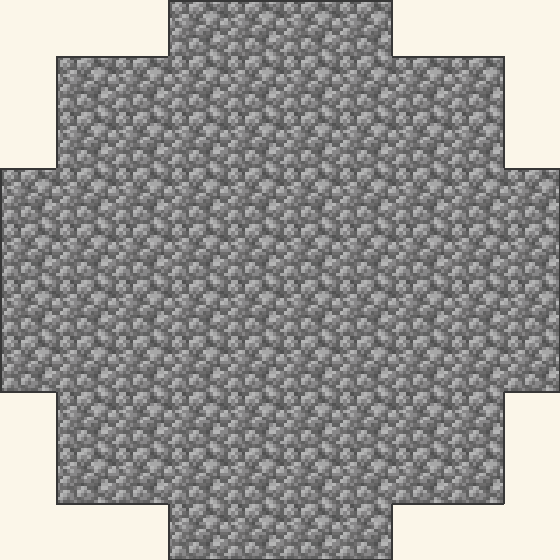
\includegraphics[width=\linewidth]{fig01_2d_d10_euclidean.png}
  \caption{\emph{Euclideo}}
\end{subfigure}\hfill
\begin{subfigure}[t]{0.31\linewidth}\centering
  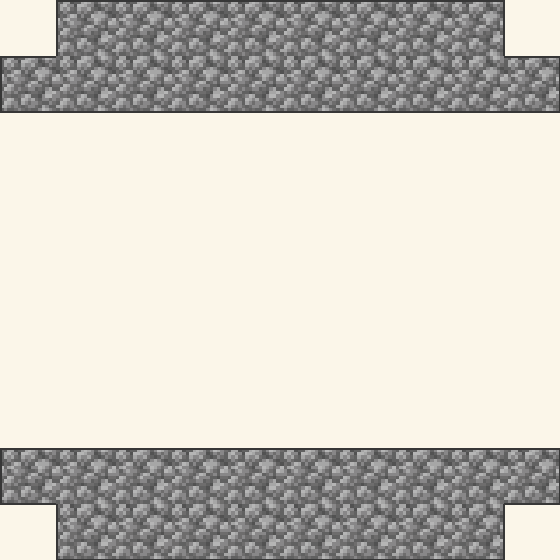
\includegraphics[width=\linewidth]{fig02_2d_d10_bresenham.png}
  \caption{\emph{Bresenham}}
\end{subfigure}\hfill
\begin{subfigure}[t]{0.31\linewidth}\centering
  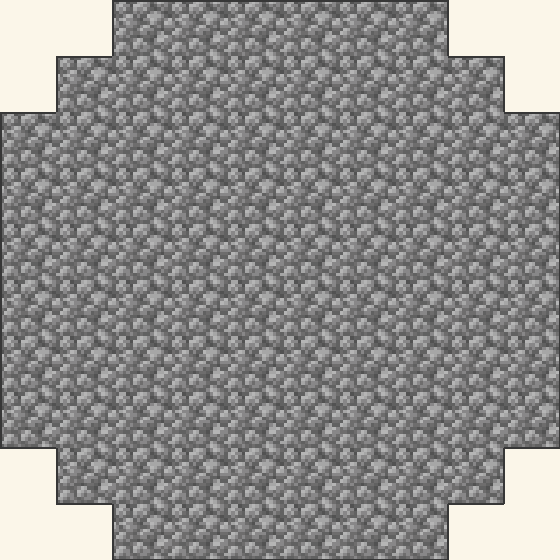
\includegraphics[width=\linewidth]{fig03_2d_d10_threshold.png}
  \caption{\emph{Umbral}}
\end{subfigure}
\caption{Misma circunferencia de diametro 10 bajo tres criterios de pertenencia, renderizada con la textura \emph{cobblestone} (piedra de canto rodado) de Minecraft. Observese como la celda de esquina, la transicion entre filas y los puntos cardinales varian de una version a otra --- son tres respuestas \emph{matematicamente correctas} bajo criterios distintos, y tres planos de construccion diferentes en \emph{Minecraft}.}
\label{fig:comp-d10}
\end{figure}

\begin{nota}[Equidad y realidad material del instituto publico]
La eleccion de Block Round responde, en parte, a un problema material concreto: la desigualdad de acceso a recursos digitales entre los institutos espanoles. La \emph{Encuesta sobre Equipamiento y Uso de TIC en los Hogares} del INE (2024) registra que mas del 95\% de los hogares con menores de 16 anos disponen de acceso a internet, pero la disparidad por nivel socioeconomico es significativa, y el equipamiento informatico en las aulas varia mucho entre comunidades autonomas. Por otro lado, el indice de posesion de \emph{smartphone} entre adolescentes de 14--18 anos supera el 95\% en todas las regiones (datos INE y Eurostat). Block Round se ha disenado precisamente para ese escenario: \emph{smartphone} economico, sin internet permanente, sin registro --- y, cuando sea necesario, el Apendice~\ref{ap:adapt-analog} ofrece un itinerario \emph{totalmente analogico} para uso exclusivo de papel cuadriculado. \emph{El propio Minecraft, en su version Bedrock movil, funciona en moviles de tres anos de uso}: el alumno puede empezar con Block Round en clase y continuar en casa con Minecraft.
\end{nota}

\begin{minecraft}[Investigacion: Minecraft en la educacion espanola]
Investigaciones recientes documentan el uso pedagogico de Minecraft en diversos centros y redes: el Instituto Nacional de Tecnologias Educativas y de Formacion del Profesorado (INTEF) mantiene materiales sobre Minecraft Education en su portal; la red XTEC (Xarxa Telematica Educativa de Catalunya) ha publicado experiencias en aulas de Secundaria; EducaMadrid y Educa.Madrid ofrecen recursos especificos para profesorado bilingue; la \emph{revista RIITE} y el congreso EDUTEC documentan casos de estudio en institutos andaluces, valencianos y vascos. La \emph{Microsoft Education Espana} mantiene un repositorio de planes de aula en castellano en \url{https://education.minecraft.net/es-es}. Esta secuencia complementa esa tradicion: usa Block Round como \emph{puente} hacia Minecraft, evitando la instalacion del juego (y la consiguiente exigencia de licencia, Java o cuenta Microsoft) en el momento de la clase.
\end{minecraft}

% =============================================================================
\section{Objetivos}\label{sec:objetivos}

\subsection{Objetivo general}

Conducir al alumnado a \acc{comprender, comparar, utilizar y traducir-en-construccion} las definiciones formales de la circunferencia, la elipse y el elipsoide como criterios de inclusion de celdas en una malla discreta de voxeles texturizados, movilizando la ecuacion implicita de esas figuras para explicar, predecir, modificar y \emph{construir en Minecraft} producciones visuales propias, en dialogo con el patrimonio cultural visual espanol (modernismo gineriano, arte geometrico, geometria nazari de la Alhambra, arquitectura de Gaudi y Calatrava) y con la tradicion matematica nacional. La consciencia de esa multiplicidad de respuestas validas conecta con una cultura matematica espanola que, desde la fundacion de la Real Sociedad Matematica Espanola (RSME, 1911) y la obra de Miguel de Guzman en la organizacion de la OME y de los congresos ICME, ha sabido conjugar rigor y divulgacion; y con una cultura ludica en la que comunidades hispanohablantes de \emph{Minecraft} ya construyen ciudades enteras articulando geometria espacial cotidianamente, sin necesariamente nombrarla.

\subsection{Objetivos especificos}

\textbf{Cognitivos (conceptuales):}
\begin{itemize}[leftmargin=1.3em,itemsep=0.2em,topsep=0.3em]
  \item identificar la ecuacion implicita $\left(\dfrac{x}{r_x}\right)^{\!2} + \left(\dfrac{y}{r_y}\right)^{\!2} = 1$ como caso general que contiene a la circunferencia $x^2 + y^2 = r^2$;
  \item reconocer que tres criterios distintos de pertenencia (distancia al centro, punto medio de Bresenham, cobertura de esquina) producen tres conjuntos diferentes de celdas --- como ya se ve en la Figura~\ref{fig:comp-d10};
  \item comprender la transicion de la ecuacion 2D a la ecuacion 3D del elipsoide y relacionarla con el calculo de volumen $V = \tfrac{4}{3}\pi r_x r_y r_z$ (asunto recurrente en la EvAU/EBAU, bloque \emph{Geometria}/\emph{Integral});
  \item interpretar el corte de un solido por un plano como una \emph{desigualdad lineal} aplicada a las coordenadas de los voxeles;
  \item comprender la \emph{aritmetica del inventario Minecraft} (\emph{stacks} de 64, cofres simples de 27 ranuras, cofres dobles de 54 ranuras) como aplicacion concreta de \emph{division con techo} y \emph{representacion de cociente y resto};
  \item identificar las \emph{simetrias} (reflexion, rotacion) que permiten construir una esfera completa a partir de un octante via \cmd{/clone} --- conexion natural con los 17 grupos de simetria plana descubiertos empiricamente en los mosaicos nazaries de la Alhambra antes de su formalizacion matematica.
\end{itemize}

\textbf{Procedimentales:}
\begin{itemize}[leftmargin=1.3em,itemsep=0.2em,topsep=0.3em]
  \item operar la interfaz de Block Round en ambos modos (2D y 3D) y exportar imagenes en PNG y \emph{schematics} en \texttt{.schem};
  \item dibujar manualmente, en papel cuadriculado, la aproximacion discreta de una circunferencia aplicando el criterio euclideo y verificarla en el software;
  \item calcular el area/volumen discreto de una figura voxelizada contando celdas y compararlo con el area/volumen continuo, expresando el resultado como error relativo;
  \item componer una figura propia combinando circulos, elipses y elipsoides con justificacion matematica de las decisiones, prediciendo el numero de bloques por tipo y la cantidad de cofres dobles necesarios;
  \item importar un \emph{schematic} exportado por Block Round en Litematica o Schematica (mods de Minecraft) y ejecutar la construccion en el juego;
  \item escribir una secuencia de comandos \cmd{/clone} que refleje 1 octante en una esfera completa.
\end{itemize}

\textbf{Actitudinales:}
\begin{itemize}[leftmargin=1.3em,itemsep=0.2em,topsep=0.3em]
  \item cooperar en parejas o trios en la produccion de las actividades practicas, simulando equipos de \emph{builders} de servidor Minecraft;
  \item argumentar matematicamente en defensa de una eleccion estetica --- competencia directamente evaluada en las pruebas EvAU/EBAU de Matematicas II y en las defensas orales de Bachillerato Internacional;
  \item reconocer que problemas reales (incluido el problema de \enquote{construir una cupula de cuarzo en el servidor del grupo}) admiten mas de una respuesta tecnicamente correcta;
  \item identificar referencias matematicas en el patrimonio cultural espanol (Alhambra, Sagrada Familia, Ciudad de las Artes y las Ciencias), en saberes ancestrales y en la produccion digital contemporanea (\emph{builders} de servidor, streamers, redes de Minecraft hispanohablantes);
  \item desarrollar \emph{etica digital}: respetar el trabajo de los companeros, citar la fuente de \emph{builds} reutilizadas, comprender el concepto de licencia.
\end{itemize}

% =============================================================================
\section{Competencias y saberes basicos LOMLOE}\label{sec:bncc}

La secuencia moviliza directamente \acc{cuatro competencias especificas} de Matematicas II del Real Decreto 217/2022, ademas de articularse con la competencia digital del Marco DigComp 2.2 y con saberes de Lenguajes, Ciencias Experimentales y Ciencias Sociales.

\begin{competencia}[Competencia especifica 1 --- Matematicas II]
Modelar y resolver problemas de la vida cotidiana y de la ciencia y la tecnologia aplicando \acc{diferentes estrategias y formas de razonamiento} para explorar distintas situaciones y obtener posibles soluciones.
\end{competencia}

\begin{competencia}[Competencia especifica 2 --- Matematicas II]
Verificar la validez de las posibles soluciones de un problema empleando el \acc{razonamiento y la argumentacion} para contrastar su idoneidad.
\end{competencia}

\begin{competencia}[Competencia especifica 4 --- Matematicas II]
Utilizar el \acc{pensamiento computacional} de forma eficaz, modificando, creando y generalizando algoritmos que resuelvan problemas mediante el uso de las matematicas, para modelizar y resolver situaciones de la vida cotidiana y del ambito de la ciencia y la tecnologia.
\end{competencia}

\begin{competencia}[Competencia especifica 7 --- Matematicas II]
Representar conceptos, procedimientos e informacion matematicos seleccionando diferentes \acc{tecnologias}, para visualizar ideas y estructurar procesos matematicos.
\end{competencia}

\medskip
Se movilizan ademas los siguientes \emph{saberes basicos} del bloque de Geometria y Analisis de Matematicas II:

\begin{itemize}[leftmargin=1.3em,itemsep=0.15em,topsep=0.3em]
  \item \acc{Geometria analitica del espacio} --- vectores en $\mathbb{R}^3$, rectas y planos, posiciones relativas, distancias.
  \item \acc{Conicas y cuadricas} --- circunferencia, elipse, esfera, elipsoide como lugares geometricos definidos por ecuaciones implicitas.
  \item \acc{Integral definida} --- calculo de areas planas y volumenes de revolucion; la formula del volumen del elipsoide como aplicacion directa.
  \item \acc{Pensamiento computacional} (saber transversal) --- abstraccion, descomposicion, reconocimiento de patrones, algoritmizacion.
\end{itemize}

\subsection{Conexion con la EvAU/EBAU}\label{sec:enem}

Los saberes y competencias anteriores conectan con los siguientes bloques de la prueba EvAU/EBAU (Evaluacion para el Acceso a la Universidad, antiguamente Selectividad/PAU) de Matematicas II, que es de obligatoria realizacion para acceder a los grados de Ciencias, Ingenieria y Ciencias de la Salud:

\begin{itemize}[leftmargin=1.3em,itemsep=0.15em,topsep=0.3em]
  \item Bloque de \emph{Geometria}: ecuaciones de planos y rectas en el espacio, distancias y angulos, posiciones relativas. Las desigualdades lineales que definen los cortes de la Aula 3 son aplicacion directa.
  \item Bloque de \emph{Analisis}: calculo integral y aplicacion al calculo de volumenes; aproximacion de integrales por sumas de Riemann (analogo discreto de la voxelizacion).
  \item Bloque de \emph{Algebra lineal}: matrices y sistemas, base teorica de las transformaciones que permiten la simetria octaedrica.
\end{itemize}

La estructura de la EvAU varia ligeramente entre comunidades autonomas; los criterios de evaluacion estatales se publican en el portal del Ministerio de Educacion, Formacion Profesional y Deportes (MEFP) y en los portales de las consejerias autonomicas.

\subsection{Competencia digital transversal}

El Marco \acc{DigComp 2.2} de la UE, integrado por la LOMLOE como competencia clave, atraviesa toda la secuencia. Se abordan cuestiones de \emph{etica digital} (licencias de software libre \emph{vs.} propietario; la propia Mojang/Microsoft permite uso educativo gratuito de Minecraft via \emph{Education Edition}), \emph{proteccion de datos personales} (\href{https://eur-lex.europa.eu/eli/reg/2016/679/oj}{RGPD --- Reglamento UE 2016/679} y \href{https://www.boe.es/buscar/act.php?id=BOE-A-2018-16673}{LOPDGDD --- Ley Organica 3/2018}), \emph{produccion autora} (derechos sobre las creaciones del alumnado en la Aula~\ref{aula5}) y \emph{ciudadania digital} (comportamiento responsable en servidores Minecraft, prevencion del \emph{griefing} y del acoso en linea, marco de la LO 8/2021 de Proteccion Integral a la Infancia y la Adolescencia frente a la Violencia, incluida la digital).

% =============================================================================
\section{Contenidos}\label{sec:conteudos}

\subsection{Conceptuales}
\begin{itemize}[leftmargin=1.3em,itemsep=0.15em,topsep=0.3em]
  \item Plano cartesiano y sistema de coordenadas en $\mathbb{R}^2$ y $\mathbb{R}^3$; centro de una celda \emph{vs.} esquina.
  \item Ecuacion reducida de la circunferencia: $x^2 + y^2 = r^2$.
  \item Ecuacion implicita general de la elipse: $\left(\dfrac{x}{r_x}\right)^{\!2} + \left(\dfrac{y}{r_y}\right)^{\!2} = 1$.
  \item Desigualdad de pertenencia: \emph{interior, exterior} y \emph{frontera}.
  \item Ecuacion del elipsoide y de la esfera en $\mathbb{R}^3$.
  \item Volumen continuo del elipsoide: $V = \tfrac{4}{3}\pi r_x r_y r_z$ (deducible por integracion de Cavalieri o por seccion).
  \item Planos en el espacio como desigualdades lineales (operacion de corte).
  \item Vecindad de una celda (4-conexa en 2D, 6-conexa en 3D).
  \item \acc{Aritmetica del inventario Minecraft}: \emph{stacks} de 64; cofres simples (27 ranuras) y dobles (54 ranuras); division con techo $N_{\mathrm{packs}} = \lceil N/64 \rceil$.
  \item \acc{Simetria octaedrica} y el grupo $\mathbb{Z}_2^3$ de reflexiones coordenadas (subgrupo de orden 8 de $O_h$): aplicacion en construccion optimizada via \cmd{/clone}. Conexion historica con los 17 grupos de simetria plana, identificados empiricamente en los mosaicos nazaries de la Alhambra de Granada siglos antes de su formalizacion por Fedorov (1891).
\end{itemize}

\subsection{Procedimentales}
\begin{itemize}[leftmargin=1.3em,itemsep=0.15em,topsep=0.3em]
  \item Trazado manual en papel cuadriculado siguiendo un criterio explicito.
  \item Operacion de Block Round (cambio de modo, ajuste de \emph{sliders}, eleccion de algoritmo, exportacion como PNG y \texttt{.schem}).
  \item Comparacion de areas/volumenes discretos y continuos por conteo.
  \item Composicion de figuras combinadas (\emph{voxel art} autoral con fundamentacion geometrica).
  \item Importacion de \texttt{.schem} en Litematica/Schematica.
  \item Ejecucion de comandos \emph{vanilla} \cmd{/fill}, \cmd{/clone}, \cmd{/setblock} y WorldEdit \cmd{//sphere}, \cmd{//hsphere}, \cmd{//ellipsoid}.
  \item Planificacion de la recogida de recursos en modo supervivencia.
\end{itemize}

\subsection{Actitudinales}
\begin{itemize}[leftmargin=1.3em,itemsep=0.15em,topsep=0.3em]
  \item Trabajo cooperativo en parejas o trios.
  \item Argumentacion fundamentada (justificar elecciones con matematicas).
  \item Etica digital: respeto a la licencia del software, a las producciones de los companeros y a las normas del servidor Minecraft compartido.
  \item Valoracion de referencias matematicas presentes en el patrimonio espanol (Alhambra, Sagrada Familia, Ciudad de las Artes y las Ciencias, escultura de Chillida y Oteiza) y en la cultura \emph{gamer} contemporanea hispanohablante.
\end{itemize}

\subsection{Modos de renderizado y variedad de algoritmos}

Ademas de cambiar de algoritmo, Block Round ofrece tres \emph{modos de renderizado} (Relleno, Fino, Grueso) que producen visuales distintos para la misma figura geometrica, como ilustra la Figura~\ref{fig:render-modes}. En Minecraft, esos modos corresponden a tres tipos de construccion distintos: una esfera \emph{Rellena} usa todos los bloques del interior (una cupula opaca de \emph{Stone}); \emph{Fina} muestra solo la corteza (una cupula \emph{hueca}, internamente vacia para una sala o museo); \emph{Gruesa} cierra las grietas diagonales que el modo Fino deja (\emph{esencial} para cupulas de \emph{Vidrio} o \emph{Hielo} submarinas que necesitan ser estancas).

\begin{figure}[!htbp]
\centering
\begin{subfigure}[t]{0.31\linewidth}\centering
  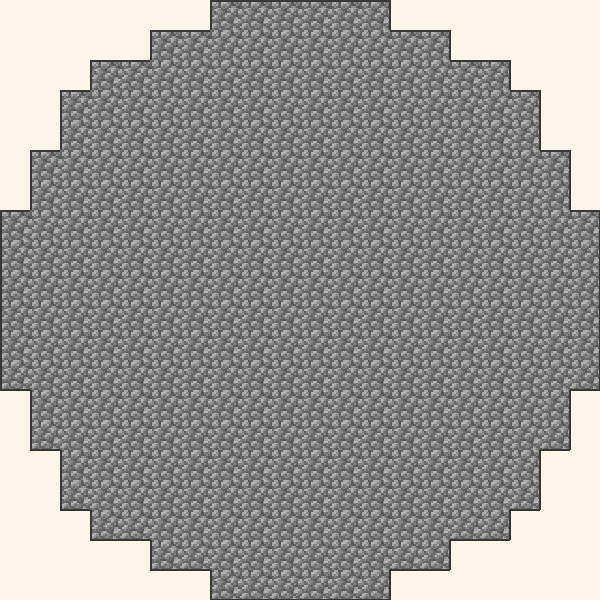
\includegraphics[width=\linewidth]{fig04_2d_d20_euclidean.png}
  \caption{\emph{Relleno}}
\end{subfigure}\hfill
\begin{subfigure}[t]{0.31\linewidth}\centering
  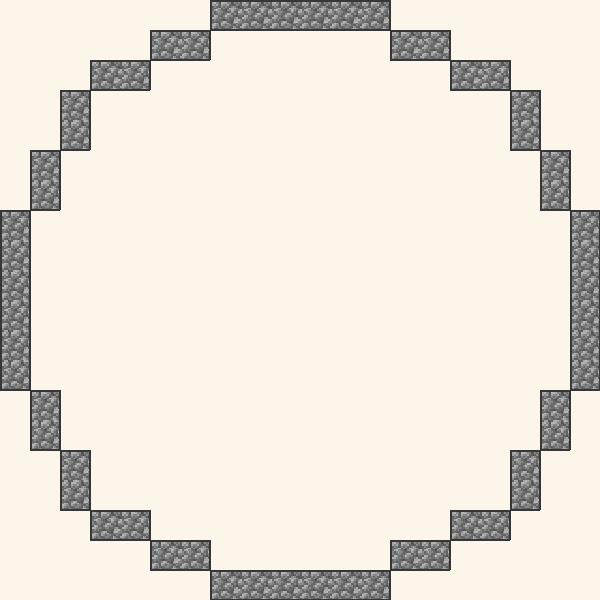
\includegraphics[width=\linewidth]{fig08_2d_d20_thin.png}
  \caption{\emph{Fino} (contorno de 1 bloque)}
\end{subfigure}\hfill
\begin{subfigure}[t]{0.31\linewidth}\centering
  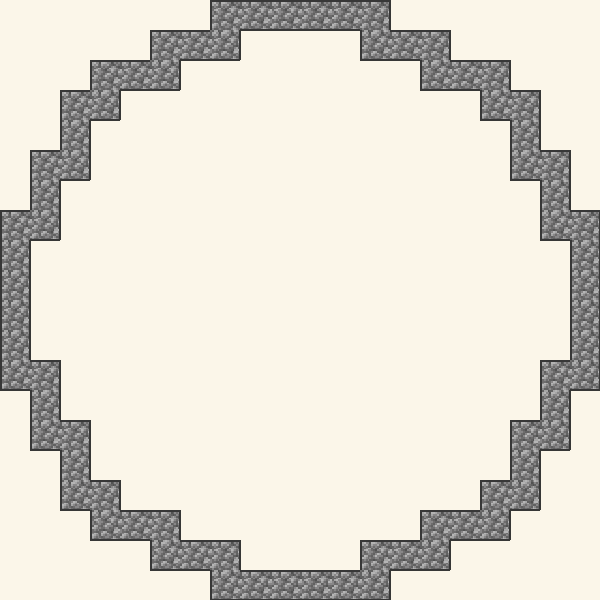
\includegraphics[width=\linewidth]{fig09_2d_d20_thick.png}
  \caption{\emph{Grueso} (contorno con puentes diagonales)}
\end{subfigure}
\caption{Los tres modos de renderizado para la misma circunferencia euclidea de diametro 20. El modo \emph{Fino} corresponde al borde discreto topologico; el modo \emph{Grueso} anade bloques en las diagonales para evitar agujeros a $45^\circ$ --- exactamente el problema que aparece en una cupula de Vidrio submarina de Minecraft, donde una grieta diagonal deja entrar el agua.}
\label{fig:render-modes}
\end{figure}

\subsection{Texturas de bloque: el diferencial Block Round}

Aunque la matematica de \emph{que voxeles colocar} es independiente de la textura, Block Round renderiza cada voxel con su textura canonica de seis caras de Minecraft. La misma esfera de diametro 10 cambia completamente de caracter visual segun el bloque elegido (Figura~\ref{fig:textures}), \emph{sin ningun cambio en el algoritmo} subyacente. Este es el punto pedagogico central: la \emph{forma} es fruto de la matematica, la \emph{apariencia} es una decision estetica posterior.

\begin{figure}[!htbp]
\centering
\begin{subfigure}[t]{0.31\linewidth}\centering
  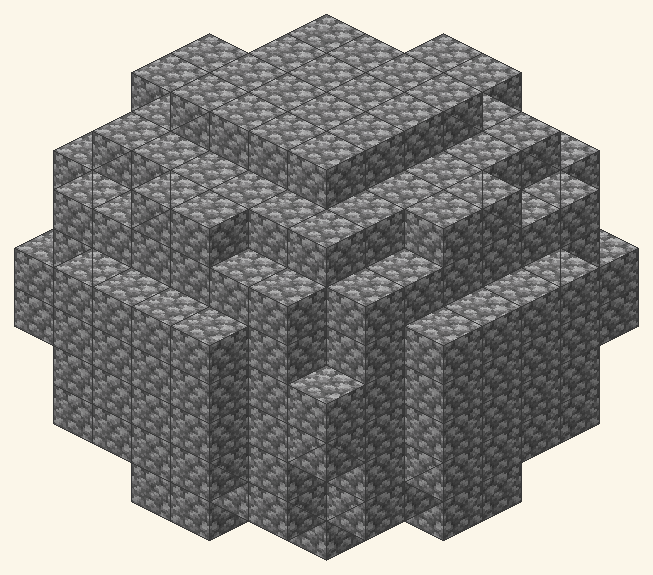
\includegraphics[width=\linewidth]{fig15_3d_sphere_cobblestone.png}
  \caption{\emph{Cobblestone}}
\end{subfigure}\hfill
\begin{subfigure}[t]{0.31\linewidth}\centering
  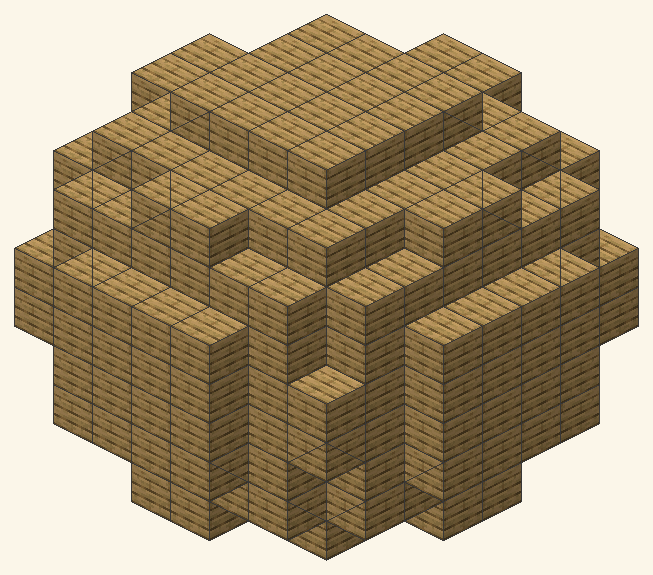
\includegraphics[width=\linewidth]{fig17_3d_sphere_oak.png}
  \caption{\emph{Oak Planks}}
\end{subfigure}\hfill
\begin{subfigure}[t]{0.31\linewidth}\centering
  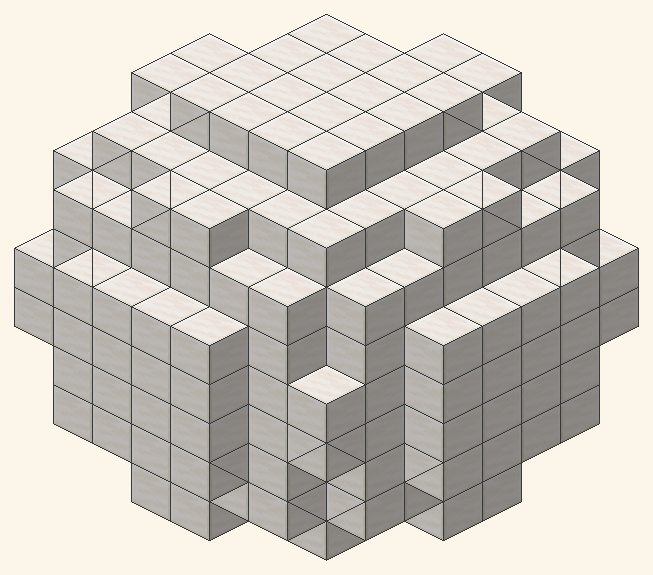
\includegraphics[width=\linewidth]{fig19_3d_sphere_quartz.png}
  \caption{\emph{Quartz Block}}
\end{subfigure}
\caption{Tres texturas de Minecraft aplicadas a la \emph{misma} esfera de diametro 10. La silueta voxelizada es identica en las tres versiones --- la matematica no ha cambiado. Lo que cambia es el caracter visual: \emph{Cobblestone} sugiere muralla medieval (Avila, Carcassonne), \emph{Oak Planks} sugiere interior de cabana o barco, \emph{Quartz Block} sugiere templo moderno o pabellon expositivo.}
\label{fig:textures}
\end{figure}

% =============================================================================
\section{Conocimientos previos}\label{sec:prerrequisitos}

La secuencia presupone contacto anterior con:

\begin{itemize}[leftmargin=1.3em,itemsep=0.15em,topsep=0.3em]
  \item Plano cartesiano: localizacion de puntos $(x, y)$ y $(x, y, z)$.
  \item Ecuacion reducida de la circunferencia (contenido de 1.\textordmasculine\ de Bachillerato).
  \item Areas de poligonos y del circulo; volumenes de cubo, prisma y cilindro (contenido de 4.\textordmasculine\ de ESO y 1.\textordmasculine\ de Bachillerato).
  \item Concepto de funcion: dominio, recorrido (imagen), grafico.
  \item Nocion de proporcion y porcentaje.
  \item Division entera con cociente y resto (contenido de ESO).
  \item Vectores en $\mathbb{R}^2$ (1.\textordmasculine\ de Bachillerato); deseable, vectores en $\mathbb{R}^3$ (2.\textordmasculine\ de Bachillerato).
\end{itemize}

\emph{Conocimiento previo opcional (no requerido, pero util):} familiaridad con Minecraft. Esta secuencia se ha disenado a proposito para que incluso alumnado que \emph{nunca} haya jugado a Minecraft (situacion poco frecuente pero posible, especialmente en colegios rurales agrupados con baja conectividad o en centros de adultos) pueda seguirla plenamente --- toda la operativa sucede en Block Round, que es \emph{autocontenido} en el navegador.

En caso de que el grupo presente desfase en alguno de los puntos obligatorios anteriores --- realidad frecuente en el contexto pos-COVID, segun los informes del INEE (Instituto Nacional de Evaluacion Educativa) y los datos de PISA 2022 que muestran caida en los indicadores de Matematicas en varias comunidades autonomas --- la \emph{Aula 1} dispone de un momento de \emph{nivelacion diagnostica} (10 min) descrito en §\ref{aula1}.

% =============================================================================
\section{Recursos y materiales}\label{sec:recursos}

\subsection{Recursos digitales}
\begin{itemize}[leftmargin=1.3em,itemsep=0.15em,topsep=0.3em]
  \item Block Round (una instancia por alumno \emph{o} por pareja);
  \item Proyector multimedia, TV con entrada HDMI o pizarra digital interactiva (PDI);
  \item Acceso a \emph{aula de informatica} \emph{o} uso de \emph{smartphones} personales (BYOD --- \emph{Bring Your Own Device}) \emph{o} \emph{tablets} distribuidas por programas autonomicos (Programa Escuela 2.0 y similares, sostenidos por las consejerias);
  \item (Opcional, Aula~\ref{aula5}) acceso a Minecraft Java Edition o Minecraft Education Edition con los mods \emph{Litematica} o \emph{Schematica} instalados; alternativamente, uso \emph{vanilla} con \cmd{/fill} y \cmd{/clone}.
\end{itemize}

\subsection{Recursos analogicos}
\begin{itemize}[leftmargin=1.3em,itemsep=0.15em,topsep=0.3em]
  \item Papel cuadriculado (1\,cm o 5\,mm), 2 hojas por alumno;
  \item Lapiz, goma, regla de 30\,cm;
  \item Lapices de colores o rotuladores (preferentemente verde-cesped \texttt{\#5B8E3F} y marron-tierra \texttt{\#825432}, paleta Block Round);
  \item Hoja de ejercicios (Apendice~\ref{ap:exerc});
  \item Pizarra convencional o pizarra blanca.
\end{itemize}

\subsection{Libro de texto y catalogo editorial}\label{sec:pnld}

Block Round complementa --- no sustituye --- al libro de texto adoptado por el centro. Los manuales de Matematicas II actualizados a LOMLOE de las principales editoriales (Anaya, SM, Santillana, Edebe, McGraw-Hill, Editex, Vicens Vives) cubren los contenidos movilizados. Capitulos especialmente relevantes:

\begin{itemize}[leftmargin=1.3em,itemsep=0.1em,topsep=0.2em,nosep]
  \item Geometria analitica del espacio: vectores, rectas, planos, distancias, posiciones relativas.
  \item Conicas: circunferencia, elipse, parabola, hiperbola (en las versiones extensas, retomadas desde 1.\textordmasculine\ Bach.).
  \item Calculo integral: integral definida; aplicacion al calculo de areas y volumenes.
  \item Algebra lineal: matrices, determinantes, sistemas (como soporte de las transformaciones lineales subyacentes a la simetria octaedrica).
\end{itemize}

Los capitulos sobre \emph{ecuacion de la circunferencia}, \emph{conicas} y \emph{geometria del espacio} (volumenes) dialogan directamente con la secuencia. En particular, problemas de \emph{teselado}, \emph{cobertura} y \emph{conteo en mallas} (comunes en los manuales) son casi identicos al problema central de Block Round, solo que con terminologia diferente.

\subsection{Acceso a Block Round}

Por orden de preferencia:

\begin{enumerate}[leftmargin=1.5em,itemsep=0.15em,topsep=0.3em]
  \item \textbf{Alojado por el profesorado} en \emph{GitHub Pages} o en el portal del centro (URL distribuida mediante codigo QR proyectado en la pizarra). Version publica: \url{https://vinisouza128.github.io/block-round/}.
  \item \textbf{Copia local} de los archivos del proyecto en una carpeta del aula de informatica, ejecutada via \emph{file://}.
  \item \textbf{Offline en \emph{smartphone}} via PWA: basta con abrir la pagina una vez con internet para que el navegador instale la aplicacion.
\end{enumerate}

% =============================================================================
\section{Adaptaciones a la realidad plural espanola}\label{sec:adapt}

El sistema educativo espanol es heterogeneo --- en parte por la transferencia competencial a las 17 comunidades autonomas y a las dos ciudades autonomas, en parte por la diversidad socioeconomica, lingueistica y cultural del pais. Esta secuencia se ha disenado para adaptarse a esa pluralidad, con variantes especificas para cada contexto.

\subsection{Instituto publico en gran ciudad}
Escenario tipico de Madrid, Barcelona, Sevilla, Valencia, Bilbao, Zaragoza, Malaga. Generalmente dispone de aula de informatica (uso compartido), pizarra digital y Wi-Fi razonable. Muchos centros estan acogidos al programa Educa.Madrid, XTEC (Catalunya), Plan Escuela TIC 2.0 (Andalucia) o equivalentes. Algunos cuentan con licencias Microsoft 365 Educacion A3 que incluyen \emph{Minecraft Education Edition} --- la Aula~\ref{aula5} puede hacerse integramente en esa version. \emph{Configuracion mas sencilla para implementar la secuencia integramente en aula de informatica.}

\subsection{Instituto publico en municipio medio o pequeno}
Realidad de la mayoria de las cabeceras de comarca y de los municipios menores de 50\,000 habitantes. El aula de informatica puede estar parcialmente operativa o compartida entre varios departamentos. Se recomienda \emph{modelo BYOD} con \emph{smartphones} personales del alumnado, organizado en parejas (un movil por pareja). Block Round funciona comodamente en \emph{Android} a partir de 2018 y en \emph{iOS} reciente. Si Minecraft no esta disponible, la Aula~\ref{aula5} puede centrarse en comandos hipoteticos (papel + descripcion del efecto) sin perder el contenido conceptual. Es la configuracion \acc{mas frecuente} en el pais.

\subsection{Centro Integrado de FP (CIFP) o Bachillerato STEM avanzado}
Red de centros publicos de excelencia tecnica (CIFP) y centros de Bachillerato con itinerario STEM reforzado, incluidos los Bachilleratos Internacionales (BI) en centros publicos. Generalmente bien equipados. La secuencia se integra de forma natural con los ciclos formativos de \emph{Desarrollo de Aplicaciones Multiplataforma} (DAM), \emph{Animaciones 3D, Juegos y Entornos Interactivos}, \emph{Sistemas Microinformaticos y Redes} (SMR) y \emph{Disenos en Fabricacion Mecanica}. Se recomienda profundizar la Aula~\ref{aula2} (algoritmo de Bresenham) con implementacion en Python en el aula de informatica, y la Aula~\ref{aula5} con la instalacion real de un servidor Minecraft Java en el laboratorio para construccion colaborativa --- frecuente en proyectos de las Escuelas Politecnicas Superiores (UPM, UPC, UPV, UPCT) que mantienen colaboracion con CIFP.

\subsection{Colegios rurales agrupados (CRA) y centros de la \enquote{Espana vaciada}}
Escenario de Teruel, Soria, Cuenca, Zamora, partes de Aragon, Castilla y Leon y Extremadura: despoblacion, conectividad limitada, plantillas docentes muy reducidas. Tradicionalmente menos equipados digitalmente, pero con \emph{fuerte conocimiento previo geometrico} de un alumnado que ha visto y manipulado geometrias agrarias (parcelas, lindes, canalizaciones de riego, eras circulares) toda su vida. Se recomienda la variante analogica (Apendice~\ref{ap:adapt-analog}) y dispositivo unico del profesor para demostracion. La Aula~\ref{aula3} puede aprovechar el conocimiento del alumnado sobre construcciones rurales circulares (eras, palomares, corrales) para articular geometria vivida y geometria simbolica. Programa Comunidad Educativa Rural (CER) y red de Centros Rurales de Innovacion Educativa (CRIE) ofrecen apoyo logistico.

\subsection{Centros con alta proporcion de alumnado gitano y de migracion reciente}
Marco de actuacion de la Estrategia Nacional para la Inclusion Social de la Poblacion Gitana 2021-2030 y de los programas PROA+ (Programa para la Orientacion, el Avance y el Enriquecimiento Educativo) del MEFP. Esta secuencia se puede \emph{enriquecer con saberes propios de la comunidad gitana} (geometria de la tradicion textil y musical) y con saberes traidos por el alumnado de migracion norteafricana, latinoamericana, subsahariana o del este de Europa (tradiciones geometricas islamicas, indigenas, ortodoxas). \emph{El profesorado de PT/AL y los mediadores interculturales son aliados esenciales en esta adaptacion}. La obra de Nuria Gorgorio (UAB) sobre matematicas y diversidad cultural ofrece un marco teorico solido. En servidor Minecraft, hay comunidades hispanohablantes que reconstruyen patrimonio cultural diverso bloque a bloque --- referenciar puede ser util.

\subsection{Educacion de Personas Adultas (EPA / CEPA / ESPA)}
Tipicamente grupos vespertinos o nocturnos, con alumnado adulto que retoma sus estudios. Block Round funciona bien aqui porque la interfaz es amigable y el tema (Minecraft / videojuegos) tambien es familiar para parte de esa franja de edad (los adultos jovenes crecieron con Minecraft a partir de 2011; otros lo conocen por sus hijos). Se sugiere reducir el tiempo de cada actividad un 20\% (debido al turno mas corto de la EPA) y priorizar discusiones orales en lugar de produccion escrita extensa. La Aula~\ref{aula5} puede hacerse \emph{opcional} en EPA, centrandose en las Aulas 1--4. Las Aulas Mentor del MEFP ofrecen un complemento de autoformacion para alumnado interesado en seguir profundizando.

\subsection{Variante para 2 sesiones dobles (100 min cada una)}
Para centros con horario en \emph{modulo doble} (frecuente en CIFP, BI y en proyectos de jornada continua): Aulas 1+2 en un modulo, 3+4 en otro, Aula 5 sola (o en modulo simple de 50 min, o en modulo doble si hay tiempo para construccion real). Total: 3 modulos de 100 min + 1 modulo de 50 min, o 2 modulos de 100 min + 1 modulo doble (200 min) para la parte practica final en Minecraft.

\subsection{Crosswalk con curriculos autonomicos}

Cada comunidad autonoma ha detallado el Real Decreto 217/2022 en su propio decreto autonomico de Bachillerato (LOMLOE). Las principales redes:

\begin{center}
\small
\begin{tabularx}{\textwidth}{@{}p{0.18\textwidth}p{0.32\textwidth}X@{}}
\toprule
\textbf{Comunidad} & \textbf{Decreto autonomico} & \textbf{Bloques relevantes (Matematicas II)} \\
\midrule
Comunidad de Madrid & Decreto 64/2022 de 27 de julio & Bloques de Geometria (analitica del espacio) y Analisis (integral, volumenes). \\
\addlinespace[3pt]
Catalunya & Decret 175/2022 (curriculum LOMLOE) & Geometria de l'espai; Analisi matematica I i II; itinerari STEAM. (Lengua vehicular: catalan.) \\
\addlinespace[3pt]
Andalucia & Orden de 30 de mayo de 2023 & Geometria espacial; aplicaciones del calculo integral; pensamiento computacional transversal. \\
\addlinespace[3pt]
Euskadi & Decreto 127/2023 de 18 de julio & Geometria del espazioa; Analisia. Curriculum trilinguee (euskara, gaztelania, ingelesa). \\
\addlinespace[3pt]
Galicia & Decreto 156/2022 de 15 de setembro & Xeometria analitica; Analise; computacion transversal. (Lengua cooficial: galego.) \\
\addlinespace[3pt]
Valencia & Decret 107/2022 de 5 d'agost & Geometria de l'espai; Analisi; itinerari cientific-tecnologic. (Lengua cooficial: valencia.) \\
\addlinespace[3pt]
Castilla y Leon & Decreto 40/2022 de 29 de septiembre & Geometria del espacio; Calculo integral; sello de calidad propio. \\
\bottomrule
\end{tabularx}
\end{center}

En las siete comunidades, los volumenes de esfera y elipsoide aparecen explicitamente en el bloque de Geometria o de Aplicaciones del Calculo Integral de Matematicas II.

\subsection{Ensenanza hibrida o remota}
La naturaleza \emph{web} de Block Round lo hace trivialmente compatible con clases remotas (Microsoft Teams, Google Meet, Zoom, plataformas autonomicas como EducaMadrid, XTEC/Moodle de Catalunya, MeducaPlus, EVAGD de Canarias, Educantabria, eVagd, eDixgal de Galicia). El profesorado comparte pantalla; el alumnado sigue en su propia maquina. Las actividades en papel cuadriculado pueden fotografiarse y enviarse como tarea asincrona via Aula Virtual del centro o WhatsApp del grupo. La Aula~\ref{aula5} puede hacerse en un servidor Minecraft compartido --- \emph{Realms} o servidor propio --- con el grupo encontrandose en el mundo virtual y construyendo colaborativamente. La experiencia acumulada en el confinamiento 2020--2021 demostro la robustez de este planteamiento.

% =============================================================================
\section{Secuencia didactica}\label{sec:sequencia}

La secuencia sigue la estructura \acc{movilizacion --- problematizacion --- sistematizacion --- sintesis}, inspirada en los \emph{tres momentos pedagogicos} de Delizoicov \& Angotti y en la tradicion de la Escuela Nueva (Giner, Luzuriaga, Sensat) de partir del conocimiento previo del alumnado. Cada sesion de 50 minutos respeta el ritmo cognitivo del adolescente, alternando momentos expositivos breves ($\leq 15$\,min) con actividades practicas.

% =============================================================================
\subsection{Aula 1 --- \enquote{?Como dibuja el juego una esfera con cubos?}}\label{aula1}

\subsubsection*{Objetivo de la sesion}
Establecer el \emph{problema central} de la rasterizacion discreta como problema matematico genuino, movilizar la ecuacion de la circunferencia y presentar Block Round. Reconocer que el problema central de la sesion --- \emph{?como decidir que bloques pintar?} --- es exactamente el problema que afronta cada jugador de Minecraft al construir una esfera en el juego.

\begin{actividad}[1.1 --- Movilizacion \quad\tempo{10 min}]
\textbf{Estrategia:} \emph{think--pair--share} (pensar individualmente, dialogar en pareja, compartir con el grupo). \\[0.4em]
\textbf{Pasos:}
\begin{enumerate}[leftmargin=1.5em,itemsep=0.2em,topsep=0.3em,nosep]
  \item Proyectar (o dibujar) tres construcciones clasicas de Minecraft: una cupula de Vidrio sobre una base de Stone (cualquier tutorial hispanohablante de YouTube --- canales como Mikecrack, Vegetta777 o La Casa de los Tres Cerditos); la \emph{Esfera Gigante} construida colectivamente en un servidor hispanohablante popular (\emph{Pretium}, \emph{Egoland}, \emph{KarmaLand} o el servidor del centro); el Pixel Art de una figura cultural espanola en Minecraft (mascota del FC Barcelona o Real Madrid, personaje de \emph{Mortadelo y Filemon}, Don Quijote, o cualquier figura significativa para el grupo).
  \item Preguntar al grupo: \emph{\enquote{Fijaos bien. ?Como decide el juego que cubos colocar para hacer una esfera? ?Tiene Minecraft un \enquote{compas magico} integrado?}}
  \item Cada alumno anota individualmente su respuesta (1\,min) y a continuacion la comenta con el companero de al lado (2\,min).
  \item Recogida colectiva: anotar respuestas-clave en una esquina de la pizarra. Conducir hacia la observacion fundamental: \emph{\enquote{El juego solo puede colocar cubos enteros --- ?como decide cuales?}}
\end{enumerate}
\end{actividad}

\begin{actividad}[1.2 --- Problematizacion \quad\tempo{15 min}]
\textbf{Estrategia:} dibujo manual confrontado con la definicion formal. \\[0.4em]
\textbf{Material:} papel cuadriculado, lapiz. \\[0.4em]
\textbf{Pasos:}
\begin{enumerate}[leftmargin=1.5em,itemsep=0.2em,topsep=0.3em,nosep]
  \item Cada alumno recibe media hoja de papel cuadriculado y marca el punto central de una region $11 \times 11$ celdas.
  \item Consigna: \emph{\enquote{Pintad el mejor circulo que podais con diametro 10 (radio 5). \emph{Imaginad que cada cuadradito es un bloque de cobblestone de Minecraft.} Teneis 4 minutos.}}
  \item Tras el tiempo, tres o cuatro alumnos pasan a la pizarra a reproducir su dibujo en una rejilla dibujada con tiza o rotulador.
  \item Observacion dirigida por el profesorado: \emph{\enquote{Mirad. ?Habeis hecho la misma figura? ?Por que no? ?Quien tiene razon? Si cada uno de vosotros estuviera construyendo esa esfera en un servidor Minecraft compartido, ?que problema generaria esto?}}
  \item Sistematizar: no hay \emph{una unica} respuesta (la Figura~\ref{fig:comp-d10} presentada en §\ref{sec:justificativa} corrobora). Cada alumno ha adoptado implicitamente un \acc{criterio} distinto para decidir si una celda entra o no.
\end{enumerate}

\textbf{Nota etnomatematica:} aprovechar el momento para mencionar que \emph{esa diversidad de respuestas es exactamente el objeto de la Etnomatematica} (Ubiratan D'Ambrosio), campo internacional reconocido por la RSME y la SEIEM (Sociedad Espanola de Investigacion en Educacion Matematica), que estudia como diferentes culturas y grupos resuelven problemas matematicos de maneras distintas e igualmente validas. \emph{La propia comunidad espanola de Minecraft constituye un grupo cultural con \enquote{etnomatematica} propia}, transmitida por tutoriales en castellano en YouTube, por mods hechos por hispanohablantes, y por servidores nacionales como \emph{Pretium}, \emph{Egoland} y \emph{MinaCraft}.
\end{actividad}

\begin{actividad}[1.3 --- Sistematizacion \quad\tempo{15 min}]
\textbf{Estrategia:} exposicion dialogada con apoyo de la pizarra. \\[0.4em]
\textbf{Contenido:}

La ecuacion implicita de la circunferencia centrada en el origen, de radio $r$, es

\begin{formula}
\centering
$\displaystyle x^2 + y^2 \;=\; r^2$
\end{formula}

Los puntos \emph{interiores} cumplen $x^2 + y^2 < r^2$; los \emph{exteriores}, $x^2 + y^2 > r^2$. La ecuacion se generaliza a la elipse de semiejes $r_x, r_y$:

\begin{formula}
\centering
$\displaystyle \left(\dfrac{x}{r_x}\right)^{\!2} + \left(\dfrac{y}{r_y}\right)^{\!2} \;=\; 1$
\end{formula}

En una malla de bloques (voxeles), el reto es decidir que \acc{celdas} pertenecen al interior. Decisiones diferentes generan dibujos diferentes. Block Round implementa \emph{tres} criterios:

\begin{itemize}[leftmargin=1.3em,itemsep=0.15em,topsep=0.3em]
  \item \acc{Euclideo}: ?el centro $(i + \tfrac{1}{2},\, j + \tfrac{1}{2})$ de la celda esta dentro?
  \item \acc{Bresenham}: algoritmo historico de 1965, opera solo con enteros.
  \item \acc{Umbral}: ?alguna \emph{esquina} de la celda esta dentro?
\end{itemize}

\textbf{Demostracion:} el profesor abre Block Round, ajusta el diametro a 10, alterna entre los tres algoritmos con el grupo observando las diferencias. Subrayar: las tres figuras son \emph{matematicamente correctas} bajo criterios distintos. Mostrar que la aplicacion permite cambiar la textura del bloque --- la esfera pasa a ser de cobblestone, oak\_planks, diamond, glowstone, y la forma \emph{no cambia}. \emph{Ese es el punto central de Block Round: la forma es matematica, la textura es eleccion estetica.}
\end{actividad}

\begin{actividad}[1.4 --- Sintesis \quad\tempo{10 min}]
\textbf{Estrategia:} aplicacion inmediata individual. \\[0.4em]
\textbf{Consigna:} \emph{\enquote{Volved al papel. Rehaced el circulo de diametro 10 aplicando \acc{rigurosamente} el criterio euclideo: pintar la celda si, y solo si, el punto central de la misma $(i + 0{,}5,\, j + 0{,}5)$ esta a una distancia menor o igual a 5 del centro.}}

Al final, comparar el dibujo del papel con lo que Block Round produce con el algoritmo Euclideo y diametro 10 --- la referencia visual es la Figura~\ref{fig:comp-d10}~(a). \emph{Deben coincidir.}
\end{actividad}

\begin{minecraft}[Conexion con el juego]
En \emph{Minecraft Java Edition} con el mod WorldEdit instalado, el comando \cmd{//sphere stone 5} dibuja exactamente la misma figura que Block Round produce con el algoritmo \emph{Bresenham} y diametro 10. El alumnado que juegue en servidores puede confirmarlo en casa --- las construcciones son identicas. \emph{Es decir: lo que estamos estudiando en clase no es una simulacion didactica de Minecraft; es la misma matematica que el juego utiliza.}
\end{minecraft}

\subsubsection*{Tarea para casa (opcional)}
Repetir el ejercicio 1.4 con diametros 8 y 14. Traer los tres dibujos en la siguiente sesion. Para quienes jueguen a Minecraft en casa: intentar reproducir el dibujo directamente en el juego (con \cmd{/setblock} bloque a bloque, o con \cmd{//sphere} si tienen WorldEdit) y fotografiar la construccion.

% =============================================================================
\subsection{Aula 2 --- \enquote{Tres algoritmos, tres dibujos, tres planos de construccion}}\label{aula2}

\subsubsection*{Objetivo de la sesion}
Profundizar en la comprension de los tres algoritmos como definiciones matematicas distintas y comparar cuantitativamente los resultados, incluido el impacto practico en terminos de \emph{numero de bloques a recoger} para un constructor de \emph{survival}.

\begin{actividad}[2.1 --- Retomada \quad\tempo{5 min}]
Recoger rapidamente los dibujos de la tarea de casa, observar variaciones en el grupo, anunciar el objetivo: \emph{\enquote{Hoy vamos a mirar cada uno de los tres algoritmos con lupa, y a descubrir por que Bresenham se considera una joya de la Computacion --- y por que la comunidad Minecraft hispanohablante, sin haber oido hablar nunca de el, ya lo usa cada dia.}}
\end{actividad}

\begin{actividad}[2.2 --- Algoritmo Euclideo \quad\tempo{10 min}]
Formalizacion. Para una celda $(i, j)$, calcular las coordenadas normalizadas

\begin{formula}
\centering
$\displaystyle d_x = \dfrac{i + \tfrac{1}{2} - c_x}{r_x},\qquad d_y = \dfrac{j + \tfrac{1}{2} - c_y}{r_y}$
\end{formula}

La celda se pinta si, y solo si, $d_x^{\,2} + d_y^{\,2} \leq 1$.

\textbf{En la pizarra:} resolver explicitamente el caso $c_x = c_y = 5$, $r_x = r_y = 5$, celda $(2, 1)$. Se tiene $d_x = (2{,}5 - 5)/5 = -0{,}5$ y $d_y = (1{,}5 - 5)/5 = -0{,}7$, de modo que $d_x^2 + d_y^2 = 0{,}25 + 0{,}49 = 0{,}74 \leq 1$. Celda \emph{dentro}. \\

Pedir al alumnado que pruebe la celda $(0, 0)$ (?cual es el resultado?). Discutir.
\end{actividad}

\begin{actividad}[2.3 --- Algoritmo de Bresenham \quad\tempo{15 min}]\label{at:23}
\textbf{Contexto historico:} Jack Bresenham publico el algoritmo en 1965 cuando trabajaba en IBM. Antes que el, trazar una recta requeria operaciones en coma flotante --- costosas en los ordenadores de la epoca. Bresenham demostro que era posible dibujar usando \emph{solo enteros}: sumas y comparaciones. Anecdota historica: en esos mismos anos 60, la primera planta de IBM en Espana (IBM Sant Cugat, Barcelona) iniciaba operaciones, y los IBM 1401 y 1620 comenzaban a instalarse en bancos y universidades espanoles --- los algoritmos como el de Bresenham viajaban directamente del laboratorio de IBM Yorktown a la peninsula.

La version para circunferencia usa un \emph{parametro de decision} $d$. Se empieza en $(x{=}0,\, y{=}R)$ con $d_0 = 1 - R$. En cada paso por el octante $0$--$45^\circ$:

\begin{formula}
\centering
$\begin{cases}
\text{si } d < 0: & \text{siguiente: } (x{+}1,\, y),\; d \mathrel{+}= 2x+3 \\
\text{si } d \geq 0: & \text{siguiente: } (x{+}1,\, y{-}1),\; d \mathrel{+}= 2(x-y)+5
\end{cases}$
\end{formula}

\textbf{Demostracion en la pizarra:} trazar paso a paso el algoritmo para $R = 5$, anotando $x, y, d$ en cada iteracion. Los ocho octantes se obtienen por simetria. \\

\textbf{Conexion con Minecraft:} el algoritmo \cmd{//sphere} del mod \emph{WorldEdit} (Sponge, Bukkit, Paper, Fabric) implementa una variante de Bresenham 3D --- la misma matematica de 1965, ahora corriendo en millones de servidores Minecraft de todo el mundo. \emph{Lo que estais aprendiendo ahora es lo que el juego usa bajo el capo cada vez que alguien escribe \texttt{//sphere stone 8}.}

\textbf{Conexion con la OIE:} el algoritmo de Bresenham es tema clasico en pruebas de la \href{https://olimpiada-informatica.org/}{Olimpiada Informatica Espanola (OIE)}, organizada por la Sociedad Cientifica Informatica de Espana (SCIE) y vinculada a la Olimpiada Internacional de Informatica (IOI). El alumnado interesado puede ampliar a traves del material gratuito disponible en el portal de la OIE y en el material de la SCIE.

\textbf{Observacion metodologica:} si el grupo presenta dificultades con el algebra del parametro $d$, basta con presentar el algoritmo como una \emph{regla} (sin demostrar la funcion de decision). La justificacion completa esta en el documento tecnico \texttt{Block\_Round\_Math\_es-ES.pdf}, §5.
\end{actividad}

\begin{actividad}[2.4 --- Algoritmo de Umbral \quad\tempo{10 min}]
Para cada celda $(i, j)$, identificar la \emph{esquina mas cercana} al centro de la forma:

\begin{formula}
\centering
$\displaystyle n_x = \mathrm{clamp}(c_x,\, i,\, i{+}1),\qquad n_y = \mathrm{clamp}(c_y,\, j,\, j{+}1)$
\end{formula}

La celda se incluye si $\left(\dfrac{n_x - c_x}{r_x}\right)^{\!2} + \left(\dfrac{n_y - c_y}{r_y}\right)^{\!2} \leq 0{,}94$.

\textbf{?Por que $0{,}94$ y no $1$?} Empiricamente, con $1$ aparecen \enquote{espinas} de 1 bloque en los puntos cardinales. El umbral ligeramente menor elimina el artefacto. \emph{Esta es una decision de ingenieria tomada por inspeccion visual} --- un ejemplo importante de como la matematica teorica no siempre basta por si sola. En terminos del MRP (Movimiento de Renovacion Pedagogica): la \enquote{palabra final} no la tiene la formula, sino el dialogo entre teoria y practica.

\textbf{Cuando usar Umbral en Minecraft:} para cupulas y domos vistos \emph{de lejos} (templo en lo alto de una montana, mausoleo en una isla), el algoritmo Umbral produce una silueta ligeramente mas \enquote{llena} que se lee mejor a traves de la niebla y de la oclusion ambiente. Coste: $\sim$\,5--10\% mas bloques por corteza. Recomendado para proyectos en los que la estetica vista desde lejos importa mas que la economia de material.
\end{actividad}

\begin{actividad}[2.5 --- Comparacion cuantitativa \quad\tempo{10 min}]\label{at:25}
\textbf{Actividad practica en parejas.} En Block Round (o en el proyector centralizado):
\begin{enumerate}[leftmargin=1.5em,itemsep=0.15em,topsep=0.3em,nosep]
  \item Fijar diametro 20 y modo \emph{Relleno} (la Figura~\ref{fig:comp-d20} muestra el resultado esperado para cada algoritmo).
  \item Activar el \emph{Info chip} en la esquina del canvas. Anotar el area de cada uno de los tres algoritmos.
  \item Calcular el area continua: $\pi r^2 = \pi \cdot 10^2 \approx 314{,}16$.
  \item Para cada algoritmo, calcular el error relativo: $\dfrac{|\text{area discreta} - \text{area continua}|}{\text{area continua}} \times 100\%$.
  \item Ordenar los tres algoritmos del mas proximo al mas lejano del valor continuo.
  \item \emph{Conexion con Minecraft:} \enquote{\emph{Si tuvierais que construir estas tres esferas en \emph{survival}, ?cual exigiria menos viajes al almacen de cobblestone? ?Cual exigiria mas?}} La diferencia en \emph{stacks} (paquetes) de 64 bloques puede llegar a 1 paquete entero entre el algoritmo de menor area (Euclideo) y el de mayor area (Umbral).
\end{enumerate}

\textbf{Resultado esperado:} Euclideo suele quedar muy cerca (error inferior al $2\%$); Umbral sobreestima en pocos puntos porcentuales; Bresenham queda en medio. Confirmar colectivamente.
\end{actividad}

\begin{figure}[!htbp]
\centering
\begin{subfigure}[t]{0.31\linewidth}\centering
  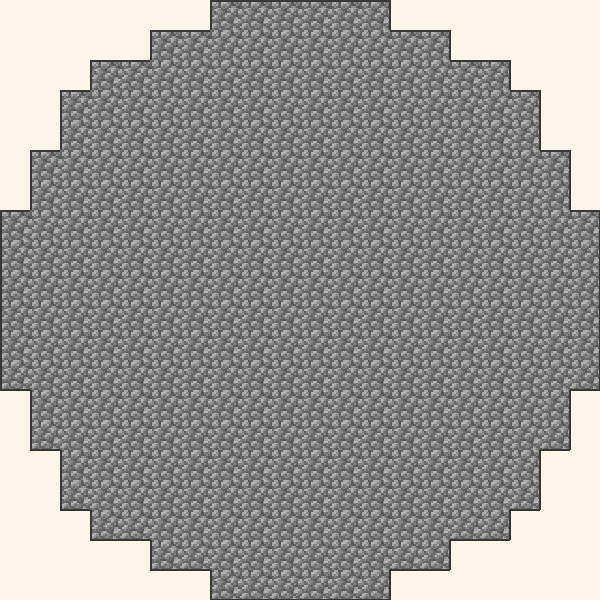
\includegraphics[width=\linewidth]{fig04_2d_d20_euclidean.png}
  \caption{\emph{Euclideo}}
\end{subfigure}\hfill
\begin{subfigure}[t]{0.31\linewidth}\centering
  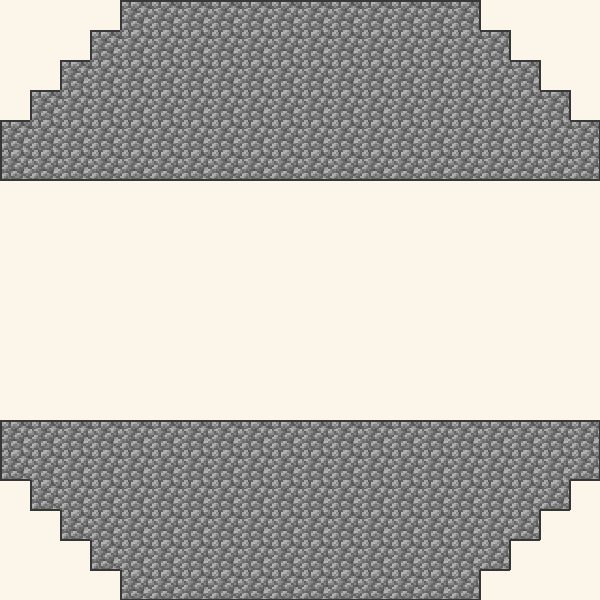
\includegraphics[width=\linewidth]{fig05_2d_d20_bresenham.png}
  \caption{\emph{Bresenham}}
\end{subfigure}\hfill
\begin{subfigure}[t]{0.31\linewidth}\centering
  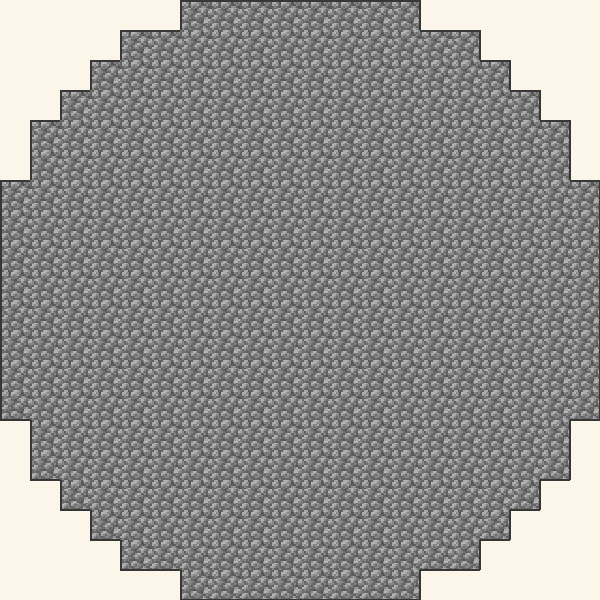
\includegraphics[width=\linewidth]{fig06_2d_d20_threshold.png}
  \caption{\emph{Umbral}}
\end{subfigure}
\caption{Misma circunferencia de diametro 20 con los tres algoritmos, renderizada con la textura cobblestone. El aumento de diametro hace las diferencias mas sutiles --- las tres versiones parecen similares a simple vista. Es un buen momento para comentar que para diametros pequenos (Figura~\ref{fig:comp-d10}) las diferencias son mucho mas evidentes.}
\label{fig:comp-d20}
\end{figure}

\begin{minecraft}[Comparacion de bloques: Block Round \emph{vs.} WorldEdit]
Probad en casa (si teneis Minecraft + WorldEdit): ejecutad \cmd{//sphere stone 10} en un servidor y contad los bloques. Comparad con lo que indica Block Round en el \emph{Info chip} para algoritmo Bresenham, $D = 20$. Los dos conteos deberian coincidir (\emph{o} diferir en 0--4 bloques por pequenas diferencias de implementacion). Si encontrais una diferencia consistente, habreis descubierto una curiosidad matematica genuina.
\end{minecraft}

% =============================================================================
\subsection{Aula 3 --- \enquote{De la elipse al elipsoide: la tercera dimension}}\label{aula3}

\subsubsection*{Objetivo de la sesion}
Generalizar la ecuacion de la elipse al elipsoide, introducir los voxeles, el calculo de volumen discreto y los cortes planares. Establecer puentes con la tradicion visual espanola y con construcciones famosas de la comunidad Minecraft hispanohablante.

\begin{actividad}[3.1 --- De la ecuacion 2D a la 3D \quad\tempo{15 min}]\label{at:31}
Anadimos una tercera coordenada $z$ al plano cartesiano. La ecuacion implicita de la elipse se generaliza de forma natural:

\begin{formula}
\centering
$\displaystyle \left(\dfrac{x}{r_x}\right)^{\!2} + \left(\dfrac{y}{r_y}\right)^{\!2} + \left(\dfrac{z}{r_z}\right)^{\!2} \;=\; 1$
\end{formula}

Cuando $r_x = r_y = r_z = r$, se recupera la \acc{esfera} $x^2 + y^2 + z^2 = r^2$, como ilustra la Figura~\ref{fig:3d-shapes}.

\textbf{Voxeles:} la celda de una malla 3D se llama \emph{voxel} (\emph{volume element}). En Minecraft, cada voxel corresponde a un \emph{bloque} de $1\times1\times1$. El criterio de pertenencia es exactamente el mismo del caso 2D, anadiendo la coordenada $z$:

\begin{formula}
\centering
$\displaystyle a_x^2 + a_y^2 + a_z^2 \leq 1,\quad \text{con } a_\xi = \dfrac{\xi + \tfrac{1}{2} - c_\xi}{r_\xi}$
\end{formula}

\textbf{Demostracion:} abrir Block Round en modo 3D, alternar entre Esfera y Elipsoide, rotar con el raton, observar la estructura de voxeles.
\end{actividad}

\begin{figure}[!htbp]
\centering
\begin{subfigure}[t]{0.45\linewidth}\centering
  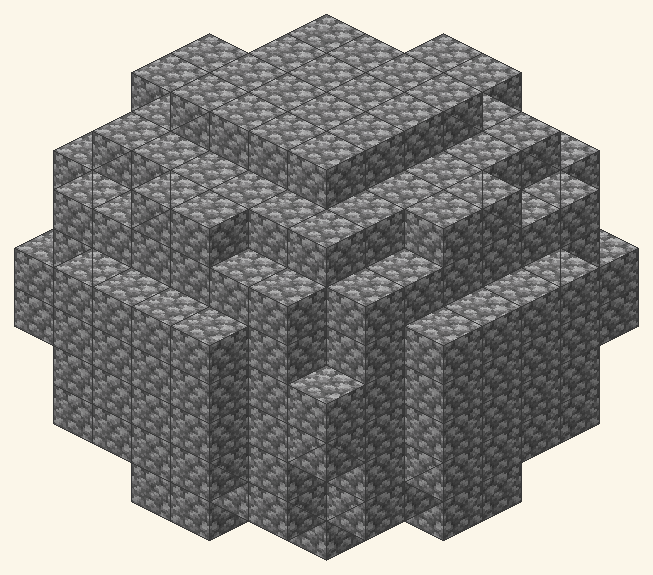
\includegraphics[width=\linewidth]{fig10_3d_sphere_d12.png}
  \caption{Esfera de diametro 10 ($r_x = r_y = r_z = 5$).}
\end{subfigure}\hfill
\begin{subfigure}[t]{0.45\linewidth}\centering
  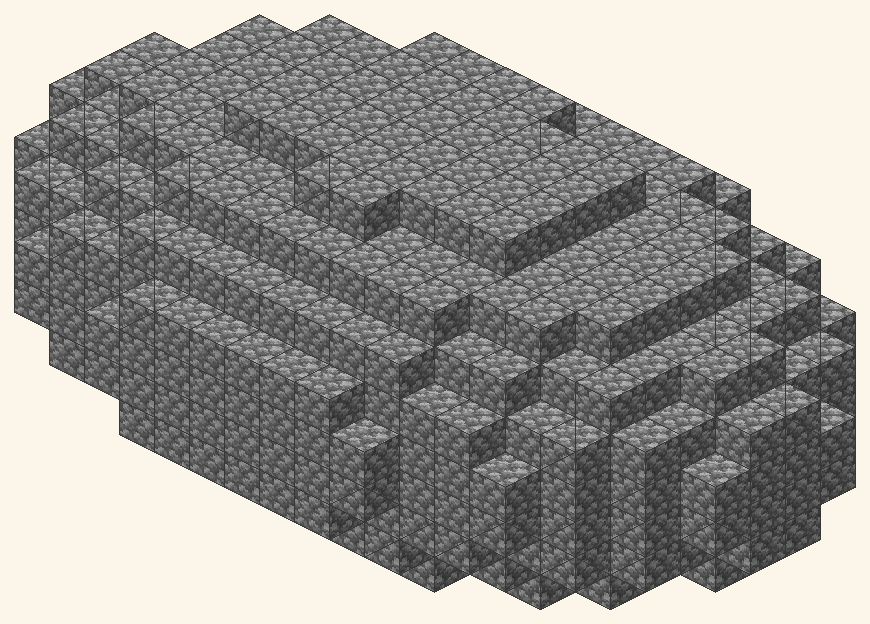
\includegraphics[width=\linewidth]{fig11_3d_ellipsoid.png}
  \caption{Elipsoide con $W = 20, H = 10, D = 12$.}
\end{subfigure}
\caption{Voxelizacion en 3D. Cada cubo es un voxel (= bloque de Minecraft); su coordenada $(i, j, k)$ en el centro se prueba en la ecuacion implicita. Las escalinatas visibles en la superficie son caracteristicas de la voxelizacion --- precisamente el aspecto que da a Minecraft su identidad visual.}
\label{fig:3d-shapes}
\end{figure}

\begin{actividad}[3.2 --- Volumen continuo \emph{vs.} discreto \quad\tempo{15 min}]\label{at:32}
El volumen continuo del elipsoide es un resultado clasico, deducible por integracion de Cavalieri:

\begin{formula}
\centering
$\displaystyle V \;=\; \dfrac{4}{3}\,\pi\, r_x\, r_y\, r_z$
\end{formula}

Cuando $r_x = r_y = r_z = r$, $V = \tfrac{4}{3}\pi r^3$. Este es un contenido \acc{recurrente en la EvAU/EBAU} (cuestiones de geometria y de aplicaciones del calculo integral aparecen en practicamente todas las convocatorias) y tambien en la fase autonomica de la \hyperref[sec:ome]{OME}, sobre todo en problemas que combinan aproximacion numerica y geometria.

\textbf{Actividad en pareja:}
\begin{enumerate}[leftmargin=1.5em,itemsep=0.15em,topsep=0.3em,nosep]
  \item Calcular el volumen continuo de una esfera de diametro 12 ($r = 6$): $V = \tfrac{4}{3}\pi \cdot 216 \approx 904{,}78$.
  \item En Block Round, generar la esfera $D = 12$, modo \emph{Relleno}, activar el \emph{Info chip}, anotar el volumen discreto (numero de bloques): aproximadamente $V_{\mathrm{disc}} \approx 904$ bloques. \emph{Error relativo $\approx 0{,}1\%$ --- impresionante.}
  \item En el mismo \emph{chip}, observar la notacion \emph{$904 = 14 \times 64 + 8$}: el juego le dice al constructor de \emph{survival} \enquote{necesitas \emph{14 stacks completos} de cobblestone + un \emph{stack} parcial con \emph{8 bloques}}.
  \item Repetir para $D = 16$ ($V_{\mathrm{cont}} \approx 2\,144$; $V_{\mathrm{disc}} \approx 2\,145$). Notar que para $D$ par el error puede incluso ser \emph{positivo} (sobreestimacion debido al centro entre celdas).
\end{enumerate}

\textbf{Observacion:} la relacion $\text{volumen discreto}/\text{volumen continuo} \to 1$ cuando $D \to \infty$. Para $D$ pequeno, hay divergencia sensible --- y matematicamente correcta: la discretizacion \emph{de hecho} altera el conteo. Esta convergencia es analoga a la convergencia de las sumas de Riemann a la integral definida, contenido central del bloque de Analisis de Matematicas II.
\end{actividad}

\begin{actividad}[3.3 --- Cortes planares \quad\tempo{10 min}]\label{at:33}
Block Round permite cortar el elipsoide por tres planos diferentes. Cada corte es una \acc{desigualdad lineal} aplicada al centro del voxel:

\begin{formula}
\centering
$\begin{array}{lcl}
\text{Eje X:} & x \geq \mathit{cut} & \Rightarrow \text{voxel descartado} \\
\text{Eje Y:} & y \geq \mathit{cut} & \Rightarrow \text{voxel descartado} \\
\text{Diagonal:} & x + y \geq \mathit{cut} & \Rightarrow \text{voxel descartado}
\end{array}$
\end{formula}

La Figura~\ref{fig:cortes} ilustra los tres cortes al $50\%$.

\textbf{Discusion dirigida:} \emph{\enquote{?Por que un corte diagonal tiene amplitud $D_x + D_y$ y no $D_x$? ?Donde esta la hipotenusa?}} Conducir hacia el reconocimiento de que $x + y$ toma valores entre $0$ y $D_x + D_y$ en la caja rectangular. \emph{En Minecraft, un corte Y 50\% en una esfera produce una \enquote{cupula} clasica --- la mitad superior de la esfera, que es exactamente la construccion que cubre templos, observatorios y arenas en miles de servidores.}
\end{actividad}

\begin{figure}[!htbp]
\centering
\begin{subfigure}[t]{0.31\linewidth}\centering
  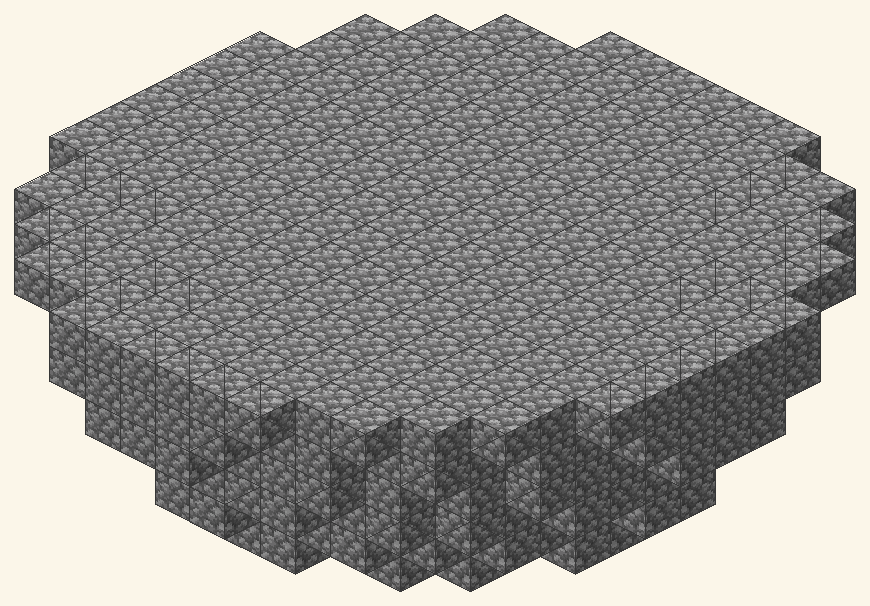
\includegraphics[width=\linewidth]{fig12_3d_cut_y50.png}
  \caption{Corte Y al 50\% --- la \emph{cupula} clasica.}
\end{subfigure}\hfill
\begin{subfigure}[t]{0.31\linewidth}\centering
  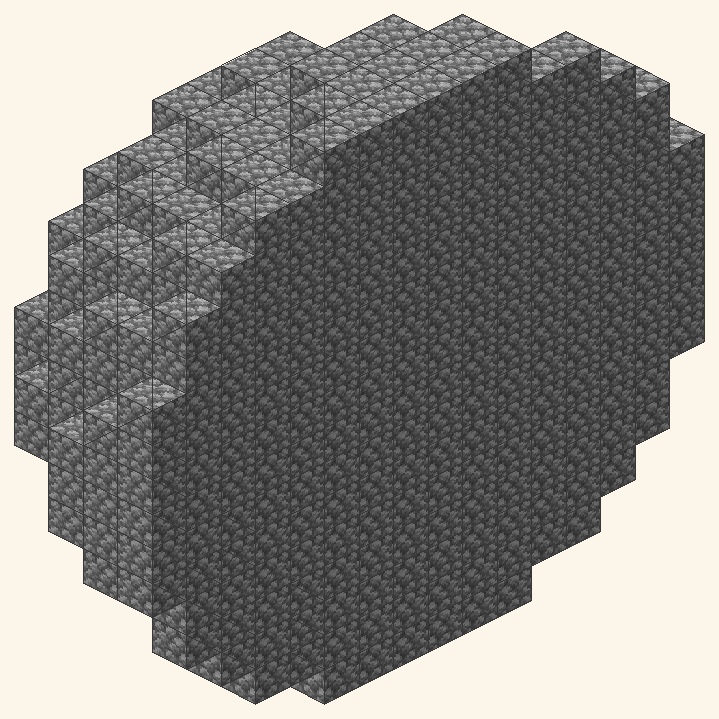
\includegraphics[width=\linewidth]{fig13_3d_cut_x50.png}
  \caption{Corte X al 50\% --- una \emph{semiesfera lateral}.}
\end{subfigure}\hfill
\begin{subfigure}[t]{0.31\linewidth}\centering
  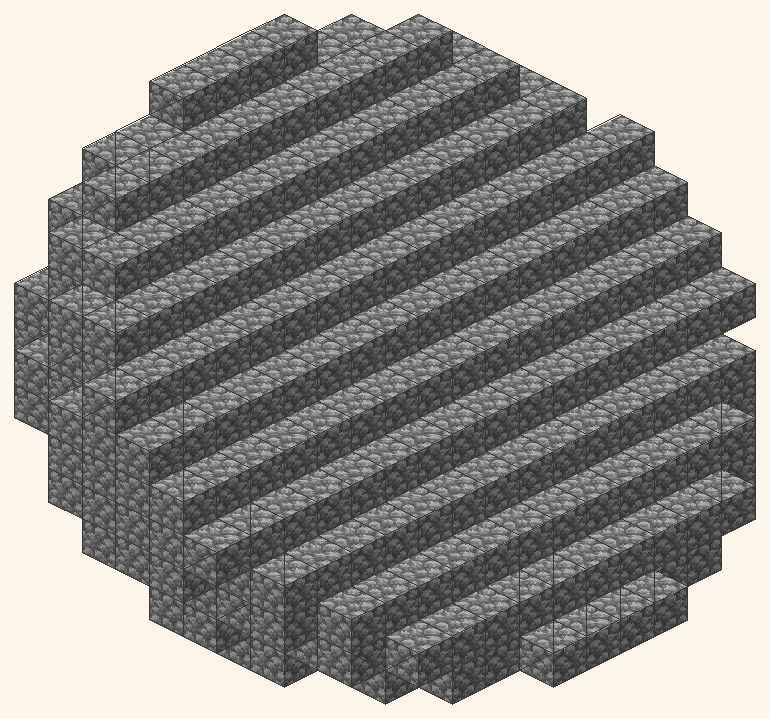
\includegraphics[width=\linewidth]{fig14_3d_cut_diag50.png}
  \caption{Corte diagonal al 50\% --- una \emph{semipiscina} oblicua.}
\end{subfigure}
\caption{Tres cortes planares en el mismo elipsoide de diametro 16, todos preservando el $50\%$ del volumen. Observese el patron escalonado caracteristico del corte diagonal: pone al descubierto la hipotenusa que conecta los dos ejes. Cada corte es un plano de construccion Minecraft distinto: cupula de templo, semiarena lateral, anfiteatro de fuente.}
\label{fig:cortes}
\end{figure}

\begin{actividad}[3.4 --- Dialogo con el patrimonio visual espanol \quad\tempo{10 min}]\label{at:34}
\emph{Conexion con Lenguajes, Arte e Historia. Esta actividad atiende las competencias clave sobre identidad cultural y patrimonio.}

Proyectar (o distribuir impresas) cinco imagenes:

\begin{itemize}[leftmargin=1.3em,itemsep=0.2em,topsep=0.3em,nosep]
  \item \acc{Sagrada Familia} (Antoni Gaudi, 1882--en obras): las columnas hiperboloides de la cripta y de la fachada de la Gloria son superficies regladas de revolucion; las boveda de la nave central usa paraboloides hiperbolicos. Gaudi llevo al concreto modernista las mismas cuadricas que estamos estudiando. La cupula central, una vez terminada, sera una de las mayores cupulas voxelizables del mundo si la tradujesemos a Minecraft.

  \item \acc{Mosaicos nazaries de la Alhambra} (Granada, ss.\ XIII--XV): la sala de los Reyes, el palacio de Comares y los patios de los Leones contienen ejemplos de los \emph{17 grupos de simetria plana} (grupos cristalograficos del plano), descubiertos empiricamente por los artesanos nazaries siglos antes de que Fedorov los formalizase matematicamente (1891) y de que Polya los popularizase en Occidente. La sequencia de teselados es \emph{voxelizacion 2D culturalmente exquisita}, y un punto de partida natural para discutir simetria octaedrica en 3D (Aula~\ref{aula4}).

  \item \acc{Talayots y navetas baleares} (II milenio a.C.): construcciones megaliticas de planta circular en Menorca y Mallorca, declaradas Patrimonio Mundial UNESCO. Geometria circular materializada en piedra siglos antes de la formalizacion griega. Junto con los castros vetones de Avila/Salamanca (poblados prerromanos de planta circular) y las pallozas asturianas y gallegas (planta circular y techo conico de paja), constituyen un patrimonio arquitectonico circular peninsular \emph{anterior al algebra} pero plenamente geometrico.

  \item \acc{Ciudad de las Artes y las Ciencias} (Santiago Calatrava, Valencia, 1998--2009): el Hemisferic es una boveda elipsoidal pura; el Palau de les Arts Reina Sofia incorpora superficies de revolucion; L'Oceanografic, disenado por Felix Candela (espanol exiliado en Mexico), usa paraboloides hiperbolicos en concreto fino. Conjunto arquitectonico que materializa exactamente las cuadricas de esta secuencia.

  \item \acc{Builds de la comunidad hispanohablante de Minecraft}: ciudades construidas en servidores como \emph{Pretium}, \emph{Egoland}, \emph{KarmaLand} o los servidores escolares de los Bachilleratos Internacionales. Se pueden mostrar \emph{timelapses} de construcciones de cupulas, esferas y arcos publicados en YouTube por Vegetta777, Willyrex, Mikecrack, AuronPlay, TheGrefg. \emph{Esta es la etnomatematica de Minecraft hispanohablante en accion}, contemporanea, viva, en castellano.
\end{itemize}

\textbf{Discusion dirigida:} \emph{\enquote{Gaudi proyecto en concreto las mismas curvas que vosotros habeis dibujado con bloques. Los artesanos nazaries representaron simetrias planas usando azulejos y yeserias --- siglos antes de que existiese el concepto formal de \emph{grupo}. Los constructores talayoticos materializaron geometrias circulares con piedra hace cuatro mil anos. La comunidad Minecraft hispanohablante lo hace en directo, cada dia, en servidores compartidos. El problema de la rasterizacion que estudiamos no es una invencion de la era digital: es una constante de la historia humana. Cada cultura ha encontrado su modo de \emph{rasterizar}.}}

\textbf{Articulacion interdisciplinar:} colaboracion sugerida con el profesorado de Dibujo Artistico, de Historia del Arte y/o de Geografia para profundizar. La Aula~\ref{aula4} y la Aula~\ref{aula5} pueden pedir a los grupos que \emph{elijan} cual tradicion visual espanola inspirara su trabajo.
\end{actividad}

% =============================================================================
\subsection{Aula 4 --- \enquote{Aritmetica del inventario: stacks, cofres, comandos}}\label{aula4}

\subsubsection*{Objetivo de la sesion}
Introducir la \emph{aritmetica de inventario} de Minecraft como aplicacion concreta de la division con techo y de la representacion de cociente y resto. Presentar los comandos centrales (\cmd{/fill}, \cmd{/clone}, \cmd{//sphere}, \cmd{//hsphere}) y la optimizacion por simetria octaedrica.

\begin{actividad}[4.1 --- Aritmetica de \emph{stacks} \quad\tempo{15 min}]\label{at:41}
En Minecraft, cada ranura del inventario lleva como maximo \acc{64 bloques identicos}. Ese limite es lo que da significado practico al calculo de volumen: $V = 904$ bloques para una esfera $D=12$ \emph{no} significa \enquote{904 en la mochila} --- significa \enquote{$\lceil 904/64 \rceil = 15$ \emph{stacks} (ranuras llenas)} de cobblestone.

\textbf{Formulas clave:}

\begin{formula}
\centering
$\displaystyle N_{\mathrm{stacks}} = \left\lceil \dfrac{V}{64} \right\rceil
\qquad\qquad
N_{\mathrm{cofres\,dobles}} = \left\lceil \dfrac{V}{3\,456} \right\rceil$
\end{formula}

(Un cofre simple tiene 27 ranuras; un cofre doble, 54 ranuras; $54 \times 64 = 3\,456$ items por cofre doble.)

\textbf{Actividad en pareja:}
\begin{enumerate}[leftmargin=1.5em,itemsep=0.15em,topsep=0.3em,nosep]
  \item Para una esfera $D = 8$ (volumen $\approx 268$ bloques): ?cuantos \emph{stacks}? ?cuantos cofres simples? Respuesta: 5 \emph{stacks}; 1 cofre simple (con 17 ranuras libres).
  \item Para una esfera $D = 16$ (volumen $\approx 2\,145$ bloques): ?cuantos \emph{stacks}? ?cuantos cofres dobles? Respuesta: 34 \emph{stacks}; 1 cofre doble (faltan 20 \emph{stacks} para llenarlo --- es decir, sobra para un cilindro pequeno mas).
  \item Para una esfera $D = 32$ (volumen $\approx 17\,156$ bloques): ?cuantos \emph{stacks}? ?cuantos cofres dobles? Respuesta: 269 \emph{stacks} (que equivalen a $\approx 5$ cofres dobles $+$ 1 \emph{stack}), $\lceil 17\,156/3\,456 \rceil = 5$ cofres dobles.
  \item \emph{En Minecraft, en modo \emph{survival}, los mineros hispanohablantes suelen extraer 1 \emph{stack} de cobblestone cada 4--6 minutos (depende del pico). Calcular el tiempo total estimado de recoleccion para la esfera $D = 16$: $34 \times 5 = 170$ minutos $\approx 2{,}8$ horas.}
\end{enumerate}
\end{actividad}

\begin{actividad}[4.2 --- Comandos Minecraft \quad\tempo{15 min}]\label{at:42}
Presentar los comandos centrales:

\begin{itemize}[leftmargin=1.4em,itemsep=0.25em,topsep=0.3em]
  \item \cmd{/setblock x y z minecraft:stone} --- coloca un bloque en una posicion especifica.
  \item \cmd{/fill x1 y1 z1 x2 y2 z2 minecraft:stone} --- rellena una caja rectangular con un bloque. Limite \emph{vanilla}: $32\,768$ bloques por comando.
  \item \cmd{/clone x1 y1 z1 x2 y2 z2 x3 y3 z3} --- copia una region a otra posicion (poder fundamental para construccion por simetria).
  \item \cmd{//sphere stone 8} (WorldEdit) --- dibuja una esfera de radio 8 centrada en el jugador, usando el algoritmo Bresenham 3D.
  \item \cmd{//hsphere stone 8} (WorldEdit) --- dibuja una esfera \emph{hueca} (solo corteza). Util para cupulas vacias por dentro.
  \item \cmd{//ellipsoid stone 10 5 10} (WorldEdit) --- elipsoide $W = 20, H = 10, D = 20$ con semiejes especificados.
\end{itemize}

\textbf{Demostracion (si hay Minecraft disponible):} ejecutar \cmd{//sphere stone 8} en un mundo de pruebas y cronometrar. Comparar con lo que Block Round muestra para diametro 16, algoritmo Bresenham. Confirmar la identidad matematica de las dos salidas.

\textbf{Si no hay Minecraft:} ejecutar mentalmente. Anotar en papel cuadriculado: \enquote{Estoy en el suelo (y=64). Quiero una esfera de radio 8 a partir de y=72 (8 bloques por encima del suelo). ?Que comando uso?} Respuesta: \cmd{//sphere stone 8} estando en $(0, 72, 0)$.
\end{actividad}

\begin{actividad}[4.3 --- Optimizacion por simetria octaedrica \quad\tempo{15 min}]\label{at:43}
\textbf{Idea central:} una esfera centrada en el origen es invariante por reflexiones en los tres planos coordenados. El grupo $\mathbb{Z}_2^3$ tiene orden 8: a partir de un \emph{octante} (region $+x, +y, +z$), las otras siete regiones se obtienen por reflexion. Esta nocion de simetria es la misma que aparece, a otra escala, en los teselados nazaries de la Alhambra: el ojo del artesano y el ojo del jugador de Minecraft realizan la misma operacion mental --- aprovechar la simetria para no repetir trabajo.

\textbf{Implicacion practica:} en lugar de colocar $V$ bloques uno a uno, construir $V/8$ bloques en el octante positivo y reflejar 7 veces con \cmd{/clone}.

\begin{formula}
\centering
$\displaystyle \mathrm{coste}_\mathrm{simetria} = N_\mathrm{octante} + 7\, T_\mathrm{clone}
\;\ll\; \mathrm{coste}_\mathrm{fuerza\,bruta} = N\, T_\mathrm{bloque}$
\end{formula}

\textbf{Ejemplo concreto, esfera $D = 24$ centrada en $(0, 72, 0)$:}
\begin{enumerate}[leftmargin=1.5em,itemsep=0.15em,topsep=0.3em,nosep]
  \item Construir manualmente el octante positivo ($\approx 905$ bloques, $\approx 15$ minutos en \emph{survival} o $\approx 45$ segundos en \emph{creative} con brocha).
  \item Reflejar en $-x$: \cmd{/clone 0 72 0 12 84 12 -12 72 0 mode:masked}
  \item Reflejar en $-y$: \cmd{/clone 0 72 0 12 84 12 0 60 0 mode:masked}
  \item Reflejar en $-z$: \cmd{/clone 0 72 0 12 84 12 0 72 -12 mode:masked}
  \item Octantes $(-x, -y)$, $(-y, -z)$, $(-x, -z)$, $(-x, -y, -z)$: comandos analogos.
\end{enumerate}

\textbf{Comparacion de tiempo:}
\begin{itemize}[leftmargin=1.3em,itemsep=0.1em,topsep=0.2em,nosep]
  \item Sin simetria, en \emph{survival}: $7\,238$ bloques $\times$ 2s/bloque $\approx$ 4 horas.
  \item Con simetria: 15 min (octante) + 0,5s (7 clones) $\approx$ 15 min.
  \item Aceleracion: \emph{factor 16}.
\end{itemize}
\end{actividad}

\begin{actividad}[4.4 --- Aplicacion: planificacion de una cupula real \quad\tempo{5 min}]
En parejas, planificar (\emph{en papel o en Block Round}) la construccion de una cupula de Quartz $D=20$ sobre un templo estilizado al gusto del grupo (referencia a Calatrava, Gaudi, Alhambra o construccion libre). Anotar:
\begin{itemize}[leftmargin=1.3em,itemsep=0.1em,topsep=0.2em,nosep]
  \item Volumen de la cupula (mitad de la esfera $D=20$): $\approx 2\,094$ bloques.
  \item \emph{Stacks} necesarios: 33 \emph{stacks}.
  \item Numero de Quartz blocks (cada uno requiere 4 Nether Quartz, minables en el Nether): $\sim 2\,094 \times 4 = 8\,376$ Nether Quartz.
  \item Secuencia de comandos optimizada usando simetria.
\end{itemize}

Esta actividad prepara el terreno para la Aula 5 (construccion real).
\end{actividad}

% =============================================================================
\subsection{Aula 5 --- \enquote{Construccion real: de Block Round a Minecraft}}\label{aula5}

\subsubsection*{Objetivo de la sesion}
Movilizar todo el contenido desarrollado en un \emph{producto autoral construido}: exportar de Block Round, importar en Minecraft (via Litematica o Schematica), ejecutar la construccion en \emph{creative} o \emph{survival}. Evaluar el aprendizaje mediante la defensa argumentativa de las decisiones matematicas y la entrega del producto final.

\begin{actividad}[5.1 --- Presentacion del reto \quad\tempo{5 min}]\label{at:51}
\textbf{Consigna:} \emph{\enquote{En parejas o trios, vais a producir una construccion en Minecraft (o en Block Round, si no hay Minecraft disponible) que combine, como minimo, tres figuras generadas por Block Round (circulos, elipses, esferas o elipsoides). Puede ser una ciudad en el servidor del grupo, un templo, una granja redonda, un observatorio --- decidis vosotros. Al final, cada grupo presentara la obra explicando \acc{matematicamente} las decisiones: ?por que ese algoritmo? ?por que esa proporcion? ?por que ese corte? ?por que esos bloques?}}
\end{actividad}

\begin{actividad}[5.2 --- Exportacion e importacion \quad\tempo{15 min}]\label{at:52}
Demostrar el flujo Block Round $\rightarrow$ Minecraft:

\begin{enumerate}[leftmargin=1.5em,itemsep=0.2em,topsep=0.3em]
  \item En Block Round, configurar la figura deseada (p.\ ej.\ esfera $D = 12$ de Quartz con \emph{cut} Y 50\%).
  \item Pulsar el boton \emph{Exportar Schematic} en la esquina del canvas. El archivo \texttt{.schem} (Sponge Schematic v2) se descarga.
  \item En Minecraft Java Edition con el mod \emph{Litematica} instalado (gratuito): abrir el mod, \emph{Load Schematic}, seleccionar el archivo descargado.
  \item Litematica muestra un \enquote{fantasma} translucido de la construccion en la posicion que el jugador elija.
  \item El jugador coloca cada bloque \emph{siguiendo al fantasma}. Litematica resalta en rojo cualquier bloque fuera de sitio.
  \item \emph{Alternativa via \cmd{//schem load}:} en servidor con WorldEdit, \cmd{//schem load nombre\_archivo} importa el \emph{schematic}, y \cmd{//paste -a} lo pega en la posicion actual --- construccion instantanea.
\end{enumerate}

\textbf{Si no hay Minecraft disponible:} demostrar la exportacion del \texttt{.schem} y exhibir el archivo binario con un editor hexadecimal --- discusion sobre el formato Sponge v2, gzip, NBT. Itinerario formativo de Tecnologia e Informatica.
\end{actividad}

\begin{actividad}[5.3 --- Produccion \quad\tempo{20 min}]\label{at:53}
\textbf{Material por grupo:}
\begin{itemize}[leftmargin=1.3em,itemsep=0.15em,topsep=0.3em,nosep]
  \item Acceso a Block Round (ordenador o \emph{smartphone});
  \item (Opcional) Acceso a Minecraft con Litematica o Schematica;
  \item Papel cuadriculado, lapiz y rotuladores para bocetos y guion;
  \item Hoja-guion con tres cuestiones obligatorias (Apendice~\ref{ap:exerc}, ejercicio 8).
\end{itemize}

\textbf{Etapas internas del trabajo de grupo:}
\begin{enumerate}[leftmargin=1.5em,itemsep=0.15em,topsep=0.3em,nosep]
  \item \tempo{5 min} \emph{Brainstorm} y boceto en papel.
  \item \tempo{8 min} Produccion en Block Round y exportacion del \texttt{.schem}.
  \item \tempo{5 min} Importacion en Minecraft y prueba rapida (si esta disponible).
  \item \tempo{2 min} Redaccion de la justificacion matematica en el guion.
\end{enumerate}

\textbf{Acompanamiento docente:} circular entre los grupos, planteando preguntas mediadoras --- \emph{\enquote{?Por que habeis elegido ese algoritmo? ?Como se podria describir ese corte mediante una desigualdad? ?Cuantos cofres dobles de Quartz vais a necesitar?}}
\end{actividad}

\begin{actividad}[5.4 --- Presentacion y sintesis colectiva \quad\tempo{10 min}]\label{at:54}
Cada grupo dispone de 2 minutos para presentar la obra al resto del grupo, mostrandola en el proyector (o en Minecraft, o fisicamente en papel) y respondiendo \emph{al menos a una} de las tres cuestiones matematicas exigidas.

\textbf{Criterios minimos de la presentacion:}
\begin{itemize}[leftmargin=1.3em,itemsep=0.1em,topsep=0.2em,nosep]
  \item identificar al menos una figura matematica presente;
  \item nombrar el algoritmo escogido y justificar (incluso \emph{a posteriori}) por que se adecua al efecto visual pretendido;
  \item si hay corte 3D, describirlo como desigualdad;
  \item estimar (aunque sea de forma aproximada) el numero de \emph{stacks}/cofres necesarios.
\end{itemize}

\textbf{Sintesis final por parte del profesorado (3 min):} retomar la idea central de la secuencia --- \emph{\enquote{en una malla discreta de voxeles, la misma curva continua admite multiples representaciones; elegir una es tomar una decision matematica; construir aquello en Minecraft es tomar una decision de ciudadania, gestion de recursos y estetica}} --- y situarla en el horizonte de la matematica espanola contemporanea: invitar al alumnado a explorar la \hyperref[sec:ome]{OME}, a participar en Estalmat, y a unirse a servidores Minecraft hispanohablantes que promueven construcciones colaborativas con valor cultural y educativo.
\end{actividad}

\begin{minecraft}[Posibilidades de ampliacion]
Esta Aula 5 abre varias posibilidades de ampliacion en proyectos extraescolares o de Bachillerato de Investigacion/Excelencia:
\begin{itemize}[leftmargin=1.3em,itemsep=0.15em,topsep=0.3em,nosep]
  \item \textbf{Proyecto Ciudad Matematica:} el grupo construye una ciudad en el servidor del centro, donde cada edificio implementa una figura geometrica (cilindro, esfera, elipsoide, conjunto de conicas).
  \item \textbf{Recreacion del patrimonio espanol:} reconstruccion en Minecraft de la Sagrada Familia, del Hemisferic de Valencia, del Guggenheim de Bilbao, de un patio de la Alhambra, de la Mezquita-Catedral de Cordoba, o de un talayot menorquin.
  \item \textbf{Olimpiada Block Round:} competicion interna --- ?quien construye la esfera mas cercana al volumen continuo? ?quien optimiza mejor el tiempo via simetria?
  \item \textbf{Articulacion con Ingenieria (UPM, UPC, UPV, escuelas de industriales):} usar Block Round como \emph{sandbox} de pre-ingenieria: cupulas geodesicas, celosias voxelizadas, estructuras que aproximan superficies suaves.
  \item \textbf{Articulacion con Programacion (OIE):} reimplementar los tres algoritmos en Python o Scratch, comparar salidas con Block Round, presentar el analisis como proyecto del Bachillerato de Investigacion o como ponencia en la Feria de la Ciencia.
\end{itemize}
\end{minecraft}

% =============================================================================
\section{Evaluacion}\label{sec:avaliacao}

La evaluacion adopta el modelo \acc{formativo}, \acc{procesual} y \acc{sumativo}, articulando cuatro dimensiones (mas una dimension especifica para la aplicacion en Minecraft) y dialogando con la tradicion espanola de la evaluacion por competencias (Neus Sanmarti, 2007; Manuel Alvarez Mendez, 2001).

\subsection{Evaluacion diagnostica}
Realizada en la Aula~\ref{aula1}, en el momento de la Actividad~1.2 (dibujo manual del circulo). Permite al profesorado identificar dificultades con el sistema de coordenadas, la ecuacion de la circunferencia y el conteo --- y solventar las lagunas pos-pandemicas evidenciadas por PISA 2022 y los informes del INEE.

\subsection{Evaluacion formativa}
Distribuida por las cinco sesiones: observacion directa de la participacion, calidad de las respuestas en el \emph{think--pair--share}, correccion \emph{inmediata} de los calculos de las Actividades~\ref{at:25}, \ref{at:32} y~\ref{at:41}.

\subsection{Evaluacion sumativa}
Compuesta por dos entregas:

\begin{enumerate}[leftmargin=1.5em,itemsep=0.2em,topsep=0.3em,nosep]
  \item \textbf{Hoja de ejercicios} (Apendice~\ref{ap:exerc}), 8 cuestiones, entregada al final de la Aula~\ref{aula5} o en la fecha acordada.
  \item \textbf{Proyecto final} (Actividad~\ref{at:53}), con guion respondido en la defensa (Actividad~\ref{at:54}).
\end{enumerate}

\subsection{Rubrica de evaluacion}

\begin{center}
\small
\begin{tabularx}{\textwidth}{@{}p{0.21\textwidth}XX@{}}
\toprule
\textbf{Dimension} & \textbf{Plenamente satisfactorio (8--10)} & \textbf{Parcialmente satisfactorio (5--7) / Insuficiente (0--4)} \\
\midrule
\textbf{Conceptos matematicos} & Aplica correctamente la ecuacion implicita de la elipse/elipsoide; reconoce los tres criterios algoritmicos y sus diferencias. & Aplica la ecuacion basica de la circunferencia pero se confunde con la generalizacion a la elipse / no reconoce las diferencias algoritmicas. \\
\addlinespace[3pt]
\textbf{Uso del software (Block Round)} & Maneja Block Round con autonomia en 2D y 3D; exporta imagenes y \texttt{.schem}; alterna algoritmos y estilos. & Necesita ayuda frecuente; opera solo en 2D. \\
\addlinespace[3pt]
\textbf{Argumentacion} & Justifica matematicamente las decisiones en el proyecto final; usa vocabulario tecnico apropiado (\emph{algoritmo}, \emph{voxel}, \emph{corte}, \emph{desigualdad}, \emph{stack}, \emph{cofre doble}). & Justifica esteticamente, sin movilizar la matematica; vocabulario ausente. \\
\addlinespace[3pt]
\textbf{Aplicacion practica Minecraft} & Calcula correctamente \emph{stacks} y cofres para el proyecto; describe secuencia de comandos \cmd{/fill} o \cmd{//sphere}; usa la simetria octaedrica. & Confunde cociente y resto; trata los bloques como unidades sueltas; no usa simetria. \\
\addlinespace[3pt]
\textbf{Cooperacion} & Trabaja productivamente en pareja/trio; contribuye al debate colectivo. & Trabaja aislado; aporta poco. \\
\bottomrule
\end{tabularx}
\end{center}

\subsection{Conversion a nota}
\begin{itemize}[leftmargin=1.3em,itemsep=0.1em,topsep=0.2em,nosep]
  \item Hoja de ejercicios: 40\% de la nota.
  \item Proyecto final + presentacion: 50\% de la nota.
  \item Observacion procesual (participacion): 10\% de la nota.
\end{itemize}

% =============================================================================
\section{Articulaciones con el ecosistema matematico espanol}\label{sec:ome}

La secuencia se inserta en un \emph{ecosistema rico} de iniciativas espanolas de educacion e investigacion en matematicas y tecnologia, que el profesorado puede movilizar como ampliacion o profundizacion.

\subsection{OME --- Olimpiada Matematica Espanola}

Fundada en 1963 y organizada por la \acc{Real Sociedad Matematica Espanola (RSME)} con el apoyo del Ministerio de Educacion, la \href{https://www.olimpiadamatematica.es/}{Olimpiada Matematica Espanola (OME)} es la mayor olimpiada de matematicas del pais y la puerta de acceso a la Olimpiada Iberoamericana y a la Olimpiada Internacional de Matematicas (IMO). Estructura clasica: fases locales (provinciales o de distrito), fase nacional, fase internacional. Miguel de Guzman Ozamiz (1936--2004) fue el principal impulsor de la OME y de la presencia espanola en la IMO, ademas de presidir el ICMI.

\emph{El contenido de esta secuencia (geometria analitica del circulo y del elipsoide, razonamiento algoritmico, aproximaciones numericas) es directamente preparatorio para los problemas de la fase nacional de la OME de nivel Bachillerato.}

\subsection{Estalmat --- Estimulo del Talento Matematico}

Iniciativa promovida por la RSME en 1998 (inspirada por Miguel de Guzman), el programa \href{https://www.estalmat.org/}{Estalmat} detecta y acompana a jovenes con talento matematico (12--16 anos) durante dos cursos sabados intensivos. Existen sedes en Madrid, Catalunya, Andalucia, Pais Vasco, Galicia, Castilla y Leon, Valencia, Canarias y otras. Esta secuencia puede ser \emph{puerta de entrada}: el alumnado que destaca en el proyecto final de la Aula~\ref{aula5} puede ser animado a presentarse a la siguiente convocatoria de Estalmat. Otros programas afines: Programa de Talento Matematico de Murcia, Beca Talento Matematico del CRM.

\subsection{Centros de investigacion matematica espanoles}

Espana no cuenta aun con medallistas Fields, pero su comunidad matematica tiene una trayectoria solida con figuras como Maria Andresa Casamayor (1720--1780, primera autora mujer de un libro de matematicas en castellano), Julio Rey Pastor, Miguel de Guzman, Jose Luis Vazquez (Premio Fonseca), Javier Cilleruelo (combinatoria aditiva, ICMAT), Pedro Luis Garcia (geometria diferencial, Universidad de Salamanca), Manuel Castellet (impulsor del CRM), Adolfo Quiros y Maria Pe Pereira (entre las nuevas generaciones).

Los principales centros de investigacion son:
\begin{itemize}[leftmargin=1.3em,itemsep=0.15em,topsep=0.3em,nosep]
  \item \acc{ICMAT} --- \href{https://www.icmat.es/}{Instituto de Ciencias Matematicas} (CSIC/UAM/UCM/UC3M), Madrid.
  \item \acc{CRM} --- \href{https://www.crm.cat/}{Centre de Recerca Matematica}, Barcelona.
  \item \acc{BCAM} --- \href{https://www.bcamath.org/}{Basque Center for Applied Mathematics}, Bilbao.
  \item \acc{IUMA} --- Instituto Universitario de Matematicas y Aplicaciones, Universidad de Zaragoza.
\end{itemize}

Sociedades cientificas: \acc{RSME} (Real Sociedad Matematica Espanola, 1911), \acc{SCM} (Societat Catalana de Matematiques), \acc{SEMA} (Sociedad Espanola de Matematica Aplicada), \acc{SEIEM} (Sociedad Espanola de Investigacion en Educacion Matematica).

\subsection{OIE --- Olimpiada Informatica Espanola}

Organizada por la Sociedad Cientifica Informatica de Espana (SCIE), la \href{https://olimpiada-informatica.org/}{OIE} tiene fases autonomicas que tradicionalmente involucran algoritmos clasicos como el de Bresenham (tratado en la Actividad~\ref{at:23}). La OIE es puerta de acceso a la Olimpiada Iberoamericana de Informatica (CIIC) y a la Olimpiada Internacional (IOI).

\subsection{Minecraft Education Edition en Espana}\label{sec:mee}

\emph{Minecraft Education Edition} es una variante educativa para centros, incluida en las licencias \emph{Microsoft 365 Educacion A1/A3} que ya despliegan varias comunidades autonomas (Comunidad de Madrid via EducaMadrid, partes de Catalunya via XTEC, Andalucia en programa piloto). Incluye recursos pedagogicos especificos (camara de pantalla, exportacion de fotos, modo \emph{Code Builder} para programacion mediante bloques visuales). \emph{Esta secuencia es compatible}: el \texttt{.schem} exportado por Block Round puede importarse tanto en Java Edition (via Litematica) como adaptarse a Education Edition (via \emph{cmdblocks} o importacion indirecta).

\subsection{Comunidades hispanohablantes de \emph{redstone engineering} y arquitectura voxel}

La comunidad hispanohablante de Minecraft mantiene canales especializados en \emph{redstone engineering} (logica computacional implementada con circuitos en el juego --- equivalente a los circuitos digitales reales) y en \emph{megaconstrucciones arquitectonicas}. Canales como \emph{Vegetta777}, \emph{Willyrex}, \emph{Mikecrack}, \emph{TheGrefg}, \emph{AuronPlay} y \emph{Rubius} (espanol-argentino) son referencias culturales que el profesorado puede aprovechar para contextualizar. Series colaborativas como \emph{KarmaLand} (Willyrex y otros), \emph{Egoland} (AuronPlay y otros) y \emph{Mineworld} marcaron a una generacion entera de jugadores hispanohablantes. \emph{Actividad complementaria:} pedir al alumnado que traiga un enlace de tutorial en castellano y analice la matematica implicita en el.

\subsection{Etnomatematica (D'Ambrosio en la tradicion espanola)}

La linea de investigacion en Etnomatematica, fundada por el brasileno \acc{Ubiratan D'Ambrosio} (1932--2021), galardonada con el ICMI Felix Klein Award (2005) --- maxima distincion mundial en Educacion Matematica ---, esta integrada en los programas de varios masteres de profesorado espanoles. La obra de Nuria Gorgorio (UAB) sobre matematicas y diversidad cultural prolonga esa linea en el contexto peninsular, especialmente en centros con alta proporcion de alumnado gitano y de migracion reciente.

\subsection{Master de Profesorado de Secundaria}

El \emph{Master en Profesorado de Educacion Secundaria Obligatoria y Bachillerato, FP e Idiomas} (especialidad Matematicas), ofrecido por todas las universidades publicas espanolas, es la via principal de formacion inicial del profesorado de Matematicas de Secundaria. El itinerario investigador del CRM (Catalunya) y del ICMAT (Madrid) ofrece continuidad para quienes quieren combinar docencia e investigacion. Esta secuencia puede servir de base para un Trabajo Fin de Master (TFM) o para un proyecto de innovacion educativa subvencionado por las consejerias autonomicas.

% =============================================================================
\section{Articulaciones interdisciplinares}\label{sec:interdisc}

\subsection{Con Dibujo Artistico, Fundamentos del Arte y Cultura Audiovisual (Lenguajes)}
La produccion de \emph{voxel art} se aborda tradicionalmente como un lenguaje artistico. Block Round ofrece una oportunidad poco frecuente de articular Matematicas y Arte sobre el mismo objeto: la figura \emph{es a la vez} una ecuacion y una composicion estetica. Sugerencia: colaboracion con el departamento de Dibujo para una exposicion final de los trabajos en el vestibulo del instituto o en las redes sociales del centro. Profundizacion posible: estudio de obras geometricas y constructivistas espanolas (Pablo Palazuelo, Equipo 57, Eduardo Chillida en escultura monumental, Jorge Oteiza en \enquote{cajas vacias} euskaras --- autenticas esculturas voxel ---, Antoni Tapies, Lluis Vives Fierro). Toda la escultura de Chillida en hierro y granito puede leerse como pre-voxelizacion.

\subsection{Con Fisica y Quimica (Ciencias Experimentales)}
La capa sonora de Block Round usa sintesis aditiva de ondas senoidales (similar a Pixel Round). Las frecuencias elegidas aproximan notas del \acc{temperamento igual de 12 tonos} (cada semitono multiplica la frecuencia por $2^{1/12} \approx 1{,}0595$). Contenido articulado con \emph{ondas mecanicas}, \emph{acustica} y \emph{funciones exponenciales}. En el contexto espanol, la musica electronica espanola pionera (Eduardo Polonio, Llorenc Barber, Carles Santos) y los laboratorios actuales de computer music en el MTG-UPF de Barcelona ofrecen referencias contemporaneas. En Minecraft, articulacion con \emph{redstone} (logica digital), \emph{notas musicales} (bloques de nota), \emph{simulacion fisica} (caida de arena, flujo de agua).

\subsection{Con Tecnologia e Informatica (itinerario STEM)}
El algoritmo de Bresenham es una referencia clasica de la Ciencia de la Computacion. Articular con clases puntuales de \emph{pensamiento computacional}: \emph{abstraccion} (la ecuacion como modelo), \emph{descomposicion} (la forma como conjunto de voxeles), \emph{reconocimiento de patrones} (simetrias), \emph{algoritmizacion} (los tres procedimientos). Conexion directa con la \hyperref[sec:ome]{OIE} y con los itinerarios formativos STEM de los Bachilleratos Internacionales y de los CIFP. La generacion del \texttt{.schem} (formato Sponge v2 con gzip + NBT) es un \emph{caso de estudio} de serializacion binaria --- contenido de los ciclos formativos de Desarrollo de Aplicaciones Multiplataforma (DAM) y de Administracion de Sistemas Informaticos en Red (ASIR). Iniciativas afines en el contexto peninsular: \emph{CSIC Code Week}, \emph{She does science}, programa STEM del CSIC, AulaDcine del MEFP.

\subsection{Con Historia e Historia del Arte (Ciencias Sociales)}
Bresenham publico el algoritmo en 1965, durante el apogeo de la computacion \emph{mainframe} en IBM. En el mismo periodo, Espana daba sus primeros pasos en computacion: los primeros IBM 1401 y 1620 llegaban a las universidades espanolas a comienzos de los anos 60 (Universidad Complutense, ETSI Telecomunicacion de Madrid, La Caixa en Barcelona); IBM Sant Cugat (Barcelona) inauguraba en 1971 la primera planta de fabricacion de IBM en la peninsula; Telefonica I+D se fundaba en 1988 como centro de investigacion aplicada. Conviene mencionar tambien a Leonardo Torres Quevedo (1852--1936), pionero universal de la automatica, que construyo \emph{El Ajedrecista} (1912), considerado el primer aut\'omata de ajedrez de la historia, y el Aerocar del Niagara. \emph{Minecraft se lanzo en 2009, se vendio a Microsoft en 2014 por 2\,500 millones de dolares y alcanzo los 300 millones de copias vendidas en 2023, convirtiendose en el videojuego mas vendido de la historia.} Su llegada al aula espanola, via partnerships Microsoft Educacion, se consolido entre 2017 y 2022.

\subsection{Con Geografia e Historia (Ciencias Sociales)}
La rasterizacion no es solo asunto del \emph{voxel art}: es la base de los \emph{sistemas de informacion geografica} (SIG/GIS). Mapas digitales del \href{https://www.ign.es/}{Instituto Geografico Nacional} (IGN), Sistema de Informacion Geografica de Parcelas Agricolas (SIGPAC) del Ministerio de Agricultura, imagenes de los satelites Sentinel del programa Copernicus de la UE, datos del INE sobre cartografia digital --- son ejemplos contemporaneos del mismo problema matematico que aborda la secuencia. \emph{Minecraft Earth} (descontinuado en 2021) fue un experimento de \emph{realidad aumentada} que superponia el universo voxel sobre mapas de ciudades reales, incluidas las espanolas.

\subsection{Con Tecnologia e Ingenieria (modalidad Ciencias y Tecnologia)}
Minecraft se usa \emph{notablemente} en escuelas tecnicas y en los CIFP como \emph{sandbox} de pre-ingenieria: el alumnado simula ciudades, sistemas electricos via \emph{redstone}, sistemas hidraulicos con agua, sistemas mecanicos con pistones y observadores. La geometria voxelizada introducida en esta secuencia es \emph{matematica de cabecera} para cualquiera que afronte \emph{Mecanica}, \emph{Resistencia de Materiales} o \emph{Estructuras}. En las Escuelas Tecnicas Superiores de Ingenieria (UPM, UPC, UPV, UPCT, US, USC, UPNA y Mondragon Unibertsitatea, entre otras), proyectos integradores con Minecraft se registran en actas de congresos como CINAIC, INRED y la SEFI Annual Conference.

% =============================================================================
\section{Referencias}\label{sec:referencias}

\subsection{Pedagogia y Educacion Matematica espanolas e iberoamericanas}
\begin{itemize}[leftmargin=1.3em,itemsep=0.15em,topsep=0.3em]
  \item ALBARRACIN, L.; GORGORIO, N. \emph{Problemas de estimacion de grandes cantidades: modelizacion e influencia del contexto}. RELIME, Revista Latinoamericana de Investigacion en Matematica Educativa, 17(3), 2014.
  \item ALVAREZ MENDEZ, J. M. \emph{Evaluar para conocer, examinar para excluir}. Madrid: Morata, 2001.
  \item BARQUERO, B.; BOSCH, M.; GASCON, J. \emph{La modelizacion matematica como herramienta didactica}. UB/UAB, varios articulos.
  \item D'AMBROSIO, U. \emph{Etnomatematica: eslabon entre las tradiciones y la modernidad}. Mexico: Limusa, 2008.
  \item GINER DE LOS RIOS, F. \emph{Estudios sobre educacion}. Madrid: Espasa-Calpe, 1933 [obra postuma; ILE].
  \item GORGORIO, N.; PLANAS, N. \emph{Cultural distance and identities-in-construction within the multicultural mathematics classroom}. ZDM, 2005.
  \item LUZURIAGA, L. \emph{Pedagogia social y politica}. Buenos Aires: Losada, 1954.
  \item MILANI, L. \emph{Carta a una maestra} [Lettera a una professoressa, 1967]. Trad.\ esp.: Barcelona: Hogar del Libro, 1970.
  \item SANMARTI, N. \emph{10 ideas clave: evaluar para aprender}. Barcelona: Grao, 2007.
  \item SENSAT, R. \emph{Vers l'escola nova}. Barcelona: Eumo, 1934 (reed.).
\end{itemize}

\subsection{Pedagogia y Educacion Matematica internacionales}
\begin{itemize}[leftmargin=1.3em,itemsep=0.15em,topsep=0.3em]
  \item DE GUZMAN, M. \emph{Aventuras matematicas}. Madrid: Piramide, 1997.
  \item FREIRE, P. \emph{Pedagogia del oprimido}. Madrid: Siglo XXI, 1970 [orig.~1968].
  \item LAKATOS, I. \emph{Pruebas y refutaciones: la logica del descubrimiento matematico}. Madrid: Alianza, 1978.
  \item POLYA, G. \emph{Como plantear y resolver problemas}. Mexico: Trillas, 1965 [orig.~1945].
  \item SKOVSMOSE, O. \emph{Educacion matematica critica: una vision sociopolitica del aprendizaje y la ensenanza de las matematicas}. Bogota: Uniandes/Una Empresa Docente, 1999.
  \item VYGOTSKI, L. S. \emph{Pensamiento y lenguaje}. Barcelona: Paidos, 1995 [orig.~1934].
\end{itemize}

\subsection{Estudios sobre videojuegos y Minecraft en la educacion}
\begin{itemize}[leftmargin=1.3em,itemsep=0.15em,topsep=0.3em]
  \item GROS, B. (coord.). \emph{Videojuegos y aprendizaje}. Barcelona: Grao, 2008.
  \item LACASA, P. \emph{Los videojuegos: aprender en mundos reales y virtuales}. Madrid: Morata, 2011.
  \item PRENSKY, M. \emph{Aprendizaje basado en juegos digitales}. Mexico: McGraw-Hill, 2011 [orig.~2001].
  \item Microsoft. \emph{Minecraft Education Edition --- portal espanol}. Disponible en \url{https://education.minecraft.net/es-es}.
  \item INTEF. \emph{Recursos educativos sobre videojuegos y gamificacion}. Ministerio de Educacion, FP y Deportes.
\end{itemize}

\subsection{Documentos oficiales}
\begin{itemize}[leftmargin=1.3em,itemsep=0.15em,topsep=0.3em]
  \item ESPANA. \href{https://www.boe.es/buscar/act.php?id=BOE-A-2020-17264}{\emph{Ley Organica 3/2020 (LOMLOE)}}. BOE 30 de diciembre de 2020.
  \item ESPANA. \href{https://www.boe.es/buscar/act.php?id=BOE-A-2022-4975}{\emph{Real Decreto 217/2022 de 29 de marzo, por el que se establece la ordenacion y las ensenanzas minimas del Bachillerato}}. BOE 30 de marzo de 2022.
  \item UNION EUROPEA. \href{https://eur-lex.europa.eu/eli/reg/2016/679/oj}{\emph{Reglamento (UE) 2016/679 (RGPD)}}. DOUE 4 de mayo de 2016.
  \item ESPANA. \href{https://www.boe.es/buscar/act.php?id=BOE-A-2018-16673}{\emph{Ley Organica 3/2018 (LOPDGDD)}}. BOE 6 de diciembre de 2018.
  \item ESPANA. \emph{Ley Organica 8/2021 de proteccion integral a la infancia y la adolescencia frente a la violencia}. BOE 5 de junio de 2021.
  \item ESPANA. \emph{Ley 4/2023 LGTBI+ para la igualdad real y efectiva}. BOE 1 de marzo de 2023.
  \item INE. \emph{Encuesta sobre Equipamiento y Uso de TIC en los Hogares 2024}. Madrid: INE.
  \item INEE. \emph{Informe espanol PISA 2022}. Madrid: MEFP.
  \item Comision Europea. \emph{Marco DigComp 2.2 --- Competencia Digital para los Ciudadanos}. Bruselas: JRC, 2022.
\end{itemize}

\subsection{Referencias tecnicas}
\begin{itemize}[leftmargin=1.3em,itemsep=0.15em,topsep=0.3em]
  \item BRESENHAM, J. E. Algorithm for computer control of a digital plotter. \emph{IBM Systems Journal}, v. 4, n. 1, p.~25--30, 1965.
  \item PITTEWAY, M. L. V. Algorithm for drawing ellipses or hyperbolae with a digital plotter. \emph{The Computer Journal}, v. 10, n. 3, p.~282--289, 1967.
  \item Sponge Schematic specification v2. \url{https://github.com/SpongePowered/Schematic-Specification}.
  \item WorldEdit documentation. \url{https://worldedit.enginehub.org}.
  \item Block Round --- documento tecnico: \texttt{docs\_math/Block\_Round\_Math\_es-ES.pdf}.
\end{itemize}

\subsection{Referencias sobre la matematica espanola}
\begin{itemize}[leftmargin=1.3em,itemsep=0.15em,topsep=0.3em]
  \item DE GUZMAN, M. \emph{El rincon de la pizarra: ensayos de visualizacion en analisis matematico}. Madrid: Piramide, 1996.
  \item RSME. \emph{La Gaceta de la RSME}. Varios numeros, \url{https://www.rsme.es/}.
  \item ICMAT. \emph{Boletin del ICMAT}. CSIC/UAM/UCM/UC3M, \url{https://www.icmat.es/}.
  \item OME. Pruebas y bancos de problemas anteriores. \url{https://www.olimpiadamatematica.es/}.
  \item GONZALEZ URBANEJA, P. M. \emph{Pitagoras: el filosofo del numero}. Madrid: Nivola, 2003. (Aproximacion divulgativa a la simetria desde la tradicion espanola de divulgacion matematica.)
  \item TORRES QUEVEDO, L. \emph{Ensayos sobre Automatica: su definicion, extension teorica de sus aplicaciones}. Revista de la Real Academia de Ciencias, 1914. (Pionero espanol de la automatica.)
\end{itemize}

\newpage
% =============================================================================
% APENDICES
% =============================================================================
\appendix
\renewcommand{\thesection}{\Alph{section}}
\setcounter{section}{0}

\section{Guion de demostracion en vivo de Block Round}\label{ap:roteiro}

Secuencia recomendada para la demostracion inicial (Actividad~1.3) y para la familiarizacion del profesorado. Tiempo total: 15 minutos.

\subsection{Apertura y modo 2D}
\begin{enumerate}[leftmargin=1.5em,itemsep=0.15em,topsep=0.3em]
  \item Abrir Block Round (\url{https://vinisouza128.github.io/block-round/}). Observar con el grupo los elementos visibles: barra superior, area central de dibujo (\emph{canvas}), controles laterales, selector de bloques debajo.
  \item Confirmar que el modo esta en \acc{2D / Circle}.
  \item Ajustar el \emph{slider} de \emph{Size} a 10. Observar la figura (comparar con la Figura~\ref{fig:comp-d10}~(a) de este plan).
  \item En la esquina inferior del canvas, activar el boton \emph{Info chip}. El grupo debe leer en voz alta: \enquote{Diameter 10, Radius 5, Blocks $\dots$, Algorithm Euclidean}.
  \item Alternar entre los tres algoritmos pulsando las \emph{pills} \acc{Euclidean} / \acc{Bresenham} / \acc{Threshold}. Detenerse en cada uno durante 30 segundos.
\end{enumerate}

\subsection{Texturas de bloque}

\begin{enumerate}[leftmargin=1.5em,itemsep=0.15em,topsep=0.3em]
  \item Mantener el diametro en 10 y el algoritmo Euclideo.
  \item Demostrar el cambio de bloque: pulsar \emph{Cobblestone}, despues \emph{Oak Planks}, despues \emph{Quartz Block}, despues \emph{Diamond}. Observar que la forma \emph{no cambia}, solo la textura.
  \item Discusion: \emph{\enquote{Estais viendo la misma esfera --- la matematica es identica. Solo cambia el vestido. En Minecraft elegis el bloque; aqui solo elegis la textura para visualizar.}}
\end{enumerate}

\needspace{18\baselineskip}
\subsection{Elipse}

\begin{figure}[!htbp]
\centering
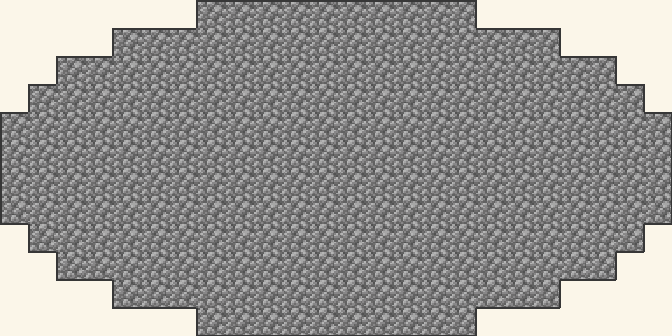
\includegraphics[width=0.45\textwidth]{fig07_2d_ellipse_24x12.png}
\caption{Elipse $W = 24, H = 12$ en Block Round. Notese que las celdas a lo largo del eje mayor estan mas espaciadas que las del eje menor.}
\label{fig:elipse}
\end{figure}

\begin{enumerate}[leftmargin=1.5em,itemsep=0.15em,topsep=0.3em]
  \item Cambiar la forma a \acc{Ellipse}. Aparecen dos \emph{sliders}: \emph{Width} y \emph{Height}.
  \item Fijar $W = 24$, $H = 12$. Observar la forma alargada --- ver Figura~\ref{fig:elipse}.
  \item Discutir: \emph{\enquote{La ecuacion que rige esta forma es $(x/12)^2 + (y/6)^2 = 1$. ?Por que dividimos $x$ entre $12$ e $y$ entre $6$?}}
\end{enumerate}

\subsection{Modo 3D, esfera y elipsoide}

\begin{enumerate}[leftmargin=1.5em,itemsep=0.15em,topsep=0.3em]
  \item Cambiar el modo a \acc{3D / Sphere}, tamano $D = 12$.
  \item Arrastrar con el raton para rotar. Aparece una esfera compuesta de voxeles.
  \item Activar el \emph{Info chip}: anotar el volumen (\enquote{904 blocks $=14 \times 64 + 8$}).
  \item Cambiar a \acc{Ellipsoid}, $W = 20$, $H = 10$, $D = 12$.
  \item Demostrar el \emph{slider Cut} en el eje \texttt{Y}, 50\% (ver Figura~\ref{fig:cortes}(a)). Observar como desaparece la mitad superior.
  \item Alternar al eje diagonal $\swarrow$/$\nearrow$ ($45^\circ$, Figura~\ref{fig:cortes}(c)). Discutir el corte oblicuo.
\end{enumerate}

\subsection{Exportacion a Minecraft}
\begin{enumerate}[leftmargin=1.5em,itemsep=0.15em,topsep=0.3em]
  \item Mostrar el boton de \emph{download} en la esquina del canvas: PNG.
  \item Mostrar el boton de \emph{export schematic}: guarda un archivo \texttt{.schem} en formato Sponge v2.
  \item Demostrar (si es posible) la importacion en Minecraft Java via mod Litematica. Ver Apendice~\ref{ap:litematica}.
\end{enumerate}

% =============================================================================
\newpage
\section{Hoja de ejercicios}\label{ap:exerc}

\textbf{Instrucciones:} responder individualmente. Se puede consultar Block Round para verificar las respuestas, \emph{pero la justificacion matematica es obligatoria}. Entregar manuscrita o mecanografiada.

\subsection*{Ejercicio 1 --- Ecuacion de la circunferencia}
\textbf{Enunciado:} Considera una circunferencia centrada en el origen $(0, 0)$ con radio $r = 7$. Verifica si cada uno de los siguientes puntos esta \emph{dentro}, \emph{fuera} o \emph{sobre} la circunferencia. Justifica con la ecuacion.
\begin{enumerate}[label=\alph*),leftmargin=1.5em,itemsep=0.1em,topsep=0.2em,nosep]
  \item $(3, 4)$ \hfill \emph{solucion:} dentro ($9 + 16 = 25 < 49$).
  \item $(5, 5)$ \hfill \emph{solucion:} \acc{fuera} ($25 + 25 = 50 > 49$, ya que $\sqrt{50} \approx 7{,}07$).
  \item $(0, 7)$ \hfill \emph{solucion:} sobre.
  \item $(-7, 0)$ \hfill \emph{solucion:} sobre.
\end{enumerate}

\textit{Atencion pedagogica:} el apartado (b) es una trampa intencionada.

\subsection*{Ejercicio 2 --- Aritmetica de \emph{stacks} y cofres}
\textbf{Enunciado:} Considera una esfera $D = 8$ en el algoritmo euclideo, con volumen continuo $V = \tfrac{4}{3}\pi \cdot 4^3 \approx 268{,}1$ y volumen discreto $V_{\mathrm{disc}} = 268$.
\begin{enumerate}[label=\alph*),leftmargin=1.5em,itemsep=0.1em,topsep=0.2em,nosep]
  \item ?Cuantos \emph{stacks} de cobblestone se necesitan para construirla? Responde en la forma $q$ \emph{stacks} $+$ $r$ bloques extra.
  \item ?Cuantos cofres simples (27 ranuras) se necesitan para almacenar todos esos \emph{stacks}?
  \item En modo \emph{survival}, suponiendo recoleccion de 1 bloque cada 0{,}5 segundos con pico de hierro, ?cuanto tiempo total de recoleccion?
\end{enumerate}

\emph{Solucion:} (a) $268 = 4 \times 64 + 12$, es decir, \acc{4 \emph{stacks} completos $+$ 12 bloques extra} (5 ranuras del inventario). (b) Basta 1 cofre simple (27 ranuras, se ocupan solo 5). (c) $268 \times 0{,}5 = 134$ segundos $\approx$ 2 min 14 s.

\subsection*{Ejercicio 3 --- Comparacion de algoritmos para D=20}
\textbf{Enunciado:} En Block Round, genera un circulo de diametro $D = 20$ con los tres algoritmos.
\begin{enumerate}[label=\alph*),leftmargin=1.5em,itemsep=0.1em,topsep=0.2em,nosep]
  \item Anota el area (numero de bloques) de cada algoritmo.
  \item ?Que algoritmo minimiza el material? ?Cual lo maximiza?
  \item ?Cual es la diferencia en \emph{stacks} entre el mayor y el menor? ?Compensa elegir el menor por economia?
\end{enumerate}

\emph{Solucion esperada:} Euclideo $\approx 316$ bloques (4 \emph{stacks} $+$ 60 extra), Bresenham $\approx 316$, Umbral $\approx 332$ bloques (5 \emph{stacks} $+$ 12 extra). Diferencia: $\approx 1$ \emph{stack}. En proyecto grande (esferas $D \geq 32$) la economia se acumula.

\subsection*{Ejercicio 4 --- Volumen de cupula y almacenamiento}
\textbf{Enunciado:} Considera una esfera $D = 16$, algoritmo Euclideo, cortada en Y al 50\% (cupula clasica).
\begin{enumerate}[label=\alph*),leftmargin=1.5em,itemsep=0.1em,topsep=0.2em,nosep]
  \item Volumen continuo de la esfera completa.
  \item Volumen de la cupula (mitad superior).
  \item ?Cuantos cofres dobles se necesitan para almacenar todos los bloques de la cupula?
  \item ?Sobra material para construir parte del suelo (una capa plana $16 \times 16$ bloques bajo la cupula)?
\end{enumerate}

\emph{Solucion:}
(a) $V = \tfrac{4}{3}\pi \cdot 8^3 \approx 2\,144{,}66$, $V_{\mathrm{disc}} \approx 2\,145$. (b) $V_{\mathrm{cupula}} \approx 1\,095$. (c) $\lceil 1\,095 / 3\,456 \rceil = 1$ cofre doble. (d) Sobra: $3\,456 - 1\,095 = 2\,361$ bloques. Suelo $16 \times 16 = 256$ bloques. Sobran 2\,105 bloques --- alcanza para el suelo y una capa adicional de banqueta.

\subsection*{Ejercicio 5 --- Elipsoide \enquote{mesa redonda gigante}}
\textbf{Enunciado:} Considera un elipsoide con $W = 24$, $H = 8$, $D = 24$ (formato aplanado tipo \enquote{mesa}).
\begin{enumerate}[label=\alph*),leftmargin=1.5em,itemsep=0.1em,topsep=0.2em,nosep]
  \item Volumen continuo.
  \item Volumen discreto estimado en Block Round.
  \item ?Sobra o falta material si has comprado 3 cofres dobles de Oak Planks?
\end{enumerate}

\emph{Solucion:}
(a) $V = \tfrac{4}{3}\pi \cdot 12 \cdot 4 \cdot 12 \approx 2\,413$.
(b) $V_{\mathrm{disc}} \approx 2\,400$ (varia $\pm 10$ segun algoritmo).
(c) Capacidad comprada: $3 \times 3\,456 = 10\,368$ bloques. Sobra mucho --- $\approx 8\,000$ bloques extra. \emph{Compra desproporcionada.} Lo ideal seria 1 cofre doble (sobra de $\approx 1\,000$ bloques).

\subsection*{Ejercicio 6 --- WorldEdit vs Block Round}
\textbf{Enunciado:} El comando WorldEdit \cmd{//sphere stone 15} usa un algoritmo similar a Bresenham 3D. Compara con la salida de Block Round en modo Bresenham con $D = 30$:
\begin{enumerate}[label=\alph*),leftmargin=1.5em,itemsep=0.1em,topsep=0.2em,nosep]
  \item ?Deberian ser identicos?
  \item Si no lo son, ?por que? Enumera al menos dos motivos.
\end{enumerate}

\emph{Solucion:}
(a) \emph{Aproximadamente si} --- ambos son Bresenham 3D, pero (b) pueden diferir por: (i) implementaciones distintas (Block Round esta en JavaScript; WorldEdit en Java); (ii) tratamiento de la paridad del diametro (par vs impar); (iii) constante empirica de \emph{threshold} (si alguno de los dos usa Umbral internamente). Diferencia tipica: 0--6 bloques para $D = 30$.

\subsection*{Ejercicio 7 --- Construccion por simetria octaedrica}
\textbf{Enunciado:} Disena la construccion de una esfera $D = 16$ centrada en $(0, 72, 0)$ en Minecraft usando simetria. Construye 1 octante (region $+x, +y, +z$, $\approx 268$ bloques) y refleja 7 veces via \cmd{/clone}.
\begin{enumerate}[label=\alph*),leftmargin=1.5em,itemsep=0.1em,topsep=0.2em,nosep]
  \item Escribe los 7 comandos \cmd{/clone} (usa \cmd{mode:masked} para no borrar el terreno).
  \item Calcula el tiempo total estimado: construccion manual del octante + comandos.
\end{enumerate}

\emph{Solucion:}

\begin{minecraft}[Secuencia de comandos]
\cmd{/clone 0 72 0 7 79 7 -8 72 0 mode:masked} \quad (reflex.\ $-x$)\\
\cmd{/clone 0 72 0 7 79 7 0 64 0 mode:masked} \quad\quad (reflex.\ $-y$)\\
\cmd{/clone 0 72 0 7 79 7 0 72 -8 mode:masked} \quad (reflex.\ $-z$)\\
\cmd{/clone -8 72 0 -1 79 7 mode:masked} \quad\quad\;\; (octante $-x,-y$)\\
\cmd{/clone 0 64 -8 7 71 -1 mode:masked} \quad\quad\;\; (octante $-y,-z$)\\
\cmd{/clone -8 72 -8 -1 79 -1 mode:masked} \quad\;\; (octante $-x,-z$)\\
\cmd{/clone -8 64 -8 -1 71 -1 mode:masked} \quad\;\; (octante $-x,-y,-z$)
\end{minecraft}

Tiempo: $\sim$\,5 min (octante manual en \emph{survival}) + $\sim$\,3 s (7 clones).

\subsection*{Ejercicio 8 --- Proyecto final}
\textbf{Enunciado:} Tras producir la construccion en grupo (Actividad~\ref{at:53}), responde:
\begin{enumerate}[label=(\arabic*),leftmargin=1.7em,itemsep=0.15em,topsep=0.2em,nosep]
  \item Enumera las figuras geometricas utilizadas (circulo, elipse, esfera, elipsoide) y sus parametros (diametro o semiejes).
  \item Para la figura principal, ?que algoritmo escogiste? ?Por que? ?Que efecto visual produce que los otros dos no produzcan?
  \item ?Hubo cortes 3D? Si los hubo, describe matematicamente \emph{uno} de ellos como desigualdad.
  \item ?Cuantos \emph{stacks}/cofres seran necesarios para construirla realmente en Minecraft en modo \emph{survival}?
  \item ?Tu produccion dialoga con alguna referencia cultural espanola (Alhambra, Gaudi, Calatrava, escultura de Chillida/Oteiza, comunidad Minecraft hispanohablante)? Comentalo.
\end{enumerate}

% =============================================================================
\newpage
\section{Adaptacion para centros sin aula de informatica}\label{ap:adapt-analog}

Esta adaptacion permite aplicar la secuencia \emph{integramente en papel} cuando el acceso a ordenador resulte inviable --- realidad frecuente en colegios rurales agrupados (CRA) de la \enquote{Espana vaciada}, centros aislados de pequenas islas baleares o canarias, y centros publicos de zonas con baja conectividad. El eje conceptual permanece intacto; lo que cambia es el soporte material.

\subsection{Sustituciones por sesion}

\begin{center}
\small
\begin{tabularx}{\textwidth}{@{}p{0.13\textwidth}p{0.32\textwidth}X@{}}
\toprule
\textbf{Sesion} & \textbf{Actividad original} & \textbf{Adaptacion analogica} \\
\midrule
1 & Demostracion de Block Round (1.3) & El profesorado dibuja a mano tres versiones de la circunferencia $D = 10$ en una rejilla preimpresa del tamano de la pizarra --- una por algoritmo. Las Figuras~\ref{fig:comp-d10} y~\ref{fig:comp-d20} pueden imprimirse como referencia. \\
\addlinespace[3pt]
2 & Comparacion cuantitativa en el software (\ref{at:25}) & Distribuir hojas con las tres circunferencias de $D = 16$ predibujadas y pedir el conteo manual. \\
\addlinespace[3pt]
3 & Generacion de la esfera 3D (\ref{at:31},~\ref{at:32}) & Distribuir hojas con \emph{rebanadas} de la esfera ($z = 0, 1, 2, \ldots$) en papel cuadriculado. El alumno construye el modelo mental por apilamiento. Cada hoja simula una \emph{capa} de bloques de Minecraft. \\
\addlinespace[3pt]
4 & Comandos Minecraft (\ref{at:42}) & Sustituir los comandos por \emph{instrucciones de construccion} escritas en castellano; el alumnado simula la ejecucion en papel cuadriculado. \\
\addlinespace[3pt]
5 & Construccion real en Minecraft (\ref{at:53}) & Construccion en \emph{LEGO} (si esta disponible), en papel cuadriculado coloreado con lapices verde-cesped y marron-tierra, o en \emph{cubos de papel} doblados por el alumnado en una clase de Plastica. \\
\bottomrule
\end{tabularx}
\end{center}

\subsection{Hojas auxiliares}
Para la version analogica completa, se recomienda preparar previamente:
\begin{itemize}[leftmargin=1.3em,itemsep=0.1em,topsep=0.2em,nosep]
  \item 1 hoja A3 con malla $30 \times 30$ dibujada con regla.
  \item 1 conjunto por alumno de 5 hojas A4 cuadriculadas (5\,mm).
  \item 1 hoja con las tres circunferencias comparativas preimpresas: las Figuras~\ref{fig:comp-d10} y~\ref{fig:comp-d20} de este plan, en A4, sirven de referencia.
  \item Para la sesion 5 analogica: 8 cubos de papel pre-doblados por grupo (representando bloques de cobblestone, oak, quartz, diamond).
\end{itemize}

\subsection{Aprovechamiento de saberes locales}
En centros rurales con fuerte tradicion artesanal (alfareria de Talavera de la Reina o de Manises, encaje de bolillos de Camarinas, ceramica murciana, damasquinado toledano, ebanisteria castellana, tejido vasco de tapices), la Aula~\ref{aula3} puede \emph{enriquecerse con una visita de portadores de saber tradicional}: alfareros, bolilleras, damasquinadores, mostrando como rasterizan circulos y simetrias en sus propios lenguajes. Esta aproximacion realiza el principio etnomatematico y dialoga con el patrimonio inmaterial reconocido por el Ministerio de Cultura. En centros con alumnado gitano o de migracion reciente, las geometrias del flamenco, del damasquinado nazari y de los patrones bereberes y andinos pueden incorporarse al debate de la Aula~\ref{aula3}.

% =============================================================================
\newpage
\section{Glosario tecnico para el profesorado}\label{ap:glos}

\begin{itemize}[leftmargin=1.4em,itemsep=0.3em,topsep=0.3em]
  \item \acc{Algoritmo} --- secuencia finita y bien definida de instrucciones para resolver un problema. Los tres algoritmos de Block Round (cf.\ Figura~\ref{fig:comp-d10}) son procedimientos distintos para el mismo problema.
  \item \acc{Bachillerato (LOMLOE)} --- etapa educativa posobligatoria de 2 cursos, regulada por el Real Decreto 217/2022; modalidades: Ciencias y Tecnologia, Humanidades y CC.\ Sociales, Artes, General.
  \item \acc{Bloque} --- unidad constructiva de Minecraft. Cubo $1\times1\times1$ con seis caras texturizadas. En lenguaje matematico, es un \emph{voxel}.
  \item \acc{Bresenham (algoritmo de)} --- algoritmo publicado en 1965 por Jack Bresenham (IBM), originalmente para recta, mas tarde extendido por otros autores (Pitteway, Kappel) para elipse. Su sena es usar \emph{solo enteros}. Vease Actividad~\ref{at:23}.
  \item \acc{Canvas} --- elemento HTML que ofrece un espacio de dibujo 2D o 3D en el navegador.
  \item \acc{Cofre (simple)} --- contenedor de Minecraft con 27 ranuras. Capacidad: $27 \times 64 = 1\,728$ items.
  \item \acc{Cofre doble} --- dos cofres adyacentes que se combinan en un contenedor de 54 ranuras. Capacidad: $54 \times 64 = 3\,456$ items.
  \item \acc{\code{/clone}} --- comando \emph{vanilla} de Minecraft que copia una region rectangular a otra posicion. Sintaxis: \cmd{/clone x1 y1 z1 x2 y2 z2 dx dy dz}. Esencial para construccion por simetria.
  \item \acc{EBAU/EvAU} --- Evaluacion para el Acceso a la Universidad (antiguamente Selectividad/PAU). Acceso a los grados universitarios.
  \item \acc{Ecuacion implicita} --- ecuacion de la forma $F(x, y) = 0$. La de la elipse: $(x/r_x)^2 + (y/r_y)^2 - 1 = 0$.
  \item \acc{Estalmat} --- programa de Estimulo del Talento Matematico promovido por la RSME desde 1998.
  \item \acc{Etnomatematica} --- campo de estudios fundado por el brasileno Ubiratan D'Ambrosio.
  \item \acc{\code{/fill}} --- comando \emph{vanilla} de Minecraft que rellena una caja rectangular con un tipo de bloque. Sintaxis: \cmd{/fill x1 y1 z1 x2 y2 z2 minecraft:stone}.
  \item \acc{ICMAT} --- Instituto de Ciencias Matematicas (CSIC/UAM/UCM/UC3M, \url{https://www.icmat.es}). Principal centro de investigacion matematica de Madrid.
  \item \acc{LOMLOE} --- Ley Organica 3/2020 de modificacion de la LOE; marco normativo educativo vigente.
  \item \acc{Litematica} --- mod popular de Minecraft Java Edition que importa \emph{schematics} y muestra un \emph{fantasma} translucido de la construccion a realizar bloque a bloque. Gratuito.
  \item \acc{LOPDGDD} --- Ley Organica 3/2018 de Proteccion de Datos Personales y Garantia de los Derechos Digitales.
  \item \acc{Minecraft Education Edition} --- version educativa de Minecraft, incluida en las licencias Microsoft 365 Educacion A1/A3 que distribuyen varias comunidades autonomas.
  \item \acc{OME} --- Olimpiada Matematica Espanola, organizada por la RSME.
  \item \acc{OIE} --- Olimpiada Informatica Espanola, organizada por la SCIE.
  \item \acc{Pack / Stack} --- pila de hasta 64 bloques identicos en una ranura del inventario de Minecraft.
  \item \acc{Pixel} --- abreviatura de \emph{picture element}. En 2D.
  \item \acc{PWA} --- \emph{Progressive Web App}. Aplicacion \emph{web} instalable y operable \emph{offline}.
  \item \acc{Rasterizacion} --- proceso de convertir una descripcion geometrica continua en una matriz de pixeles (2D) o voxeles (3D).
  \item \acc{Real Decreto 217/2022} --- norma estatal que regula la ordenacion y ensenanzas minimas del Bachillerato bajo LOMLOE.
  \item \acc{RGPD} --- Reglamento General de Proteccion de Datos (UE) 2016/679. Aplicable a toda actividad educativa con datos personales.
  \item \acc{RSME} --- Real Sociedad Matematica Espanola, fundada en 1911. Editora de \emph{La Gaceta de la RSME}.
  \item \acc{Schematica} --- mod alternativo a Litematica, con funcion similar.
  \item \acc{Schematic (\texttt{.schem})} --- formato de archivo que serializa una region de Minecraft (Sponge Schematic v2, gzip + NBT).
  \item \acc{SCIE} --- Sociedad Cientifica Informatica de Espana.
  \item \acc{Semieje} --- en una elipse, distancia del centro al extremo en la direccion del eje.
  \item \acc{\code{//sphere}} --- comando WorldEdit que construye una esfera. Sintaxis: \cmd{//sphere bloque radio}.
  \item \acc{Slot / Ranura} --- celda individual del inventario de Minecraft. Inventario completo del jugador: 36 ranuras ($9 \times 4$).
  \item \acc{Voxel} --- abreviatura de \emph{volume element}. Generalizacion del pixel a 3D. En Minecraft, cada \emph{bloque} es un voxel.
  \item \acc{WebGL} --- biblioteca de programacion grafica 3D para navegadores.
  \item \acc{WorldEdit} --- mod muy popular de Minecraft Java que anade comandos avanzados de construccion a gran escala, incluidos \cmd{//sphere}, \cmd{//hsphere}, \cmd{//ellipsoid}, \cmd{//cyl}, \cmd{//schem load}.
\end{itemize}

% =============================================================================
\newpage
\section{Tutorial: de Block Round a Minecraft via Litematica}\label{ap:litematica}

Este apendice describe el flujo completo de exportacion de Block Round e importacion en Minecraft Java Edition usando el mod \emph{Litematica}. Tiempo total esperado: 15 minutos (primera vez).

\subsection{Requisitos previos}
\begin{itemize}[leftmargin=1.3em,itemsep=0.1em,topsep=0.2em,nosep]
  \item Minecraft Java Edition (compra en la \emph{Mojang Store}; la version educativa \emph{Minecraft Education} tambien funciona, con ajustes).
  \item \emph{Fabric Loader} para la version de Minecraft que utilices (normalmente la mas reciente: \url{https://fabricmc.net/use/}).
  \item Mods: \emph{Fabric API} y \emph{Litematica} (\url{https://www.curseforge.com/minecraft/mc-mods/litematica}).
  \item Block Round abierto en el navegador, con la figura deseada ya producida.
\end{itemize}

\subsection{Paso 1: exportar desde Block Round}
\begin{enumerate}[leftmargin=1.5em,itemsep=0.15em,topsep=0.3em]
  \item En Block Round, configura la figura deseada (modo, forma, diametro, algoritmo, bloque, corte). Verifica en el \emph{Info chip} el volumen.
  \item Pulsa el boton \emph{Export Schematic} (esquina superior derecha del canvas, segundo icono). Se descarga un archivo \texttt{.schem}.
\end{enumerate}

\subsection{Paso 2: instalar Litematica}
\begin{enumerate}[leftmargin=1.5em,itemsep=0.15em,topsep=0.3em]
  \item Instala Fabric Loader en la version de Minecraft que utilices.
  \item Descarga \emph{Fabric API} y \emph{Litematica} para la misma version de Minecraft. Coloca ambos en el directorio \texttt{.minecraft/mods/}.
  \item Inicia Minecraft con el perfil \emph{fabric-loader-x.y.z-1.20.x}.
\end{enumerate}

\subsection{Paso 3: importar el schematic}
\begin{enumerate}[leftmargin=1.5em,itemsep=0.15em,topsep=0.3em]
  \item Coloca el archivo \texttt{.schem} en \texttt{.minecraft/schematics/} (o en la carpeta predeterminada de Litematica, definida en la configuracion del mod).
  \item En un mundo (creativo o supervivencia), pulsa \texttt{M} para abrir el menu de Litematica.
  \item Pulsa \emph{Load Schematic} $\rightarrow$ selecciona el archivo $\rightarrow$ \emph{Load}.
  \item El \emph{schematic} aparece ahora en una lista. Pulsalo y a \emph{Placement}: el \enquote{fantasma} translucido de la figura aparece en el mundo.
  \item Usa los controles de movimiento (\texttt{M} $\rightarrow$ \emph{Placements}) para arrastrar el fantasma a la posicion deseada. En terreno plano, basta con situar la esquina inferior $(x_1, y_1, z_1)$ en el suelo.
\end{enumerate}

\subsection{Paso 4: construir}
\begin{enumerate}[leftmargin=1.5em,itemsep=0.15em,topsep=0.3em]
  \item En \emph{Creative}: vuela sobre el fantasma y coloca cada bloque donde Litematica indique; el mod confirma con verde los bloques correctos y marca en rojo cualquier error. La construccion de una esfera $D = 12$ lleva $\approx$\,5 minutos.
  \item En \emph{Survival}: identico, pero hay que recoger los bloques antes. Usa el calculo de \emph{stacks}/cofres de la Actividad~\ref{at:41} para planificar la recoleccion.
  \item Alternativa: si el servidor tiene WorldEdit, usa \cmd{//schem load nombre-archivo} seguido de \cmd{//paste -a} para construccion instantanea.
\end{enumerate}

\subsection{Paso 5: verificacion}
Litematica resalta en rojo cualquier bloque incorrecto (faltante, del tipo equivocado o mal colocado). Usa el atajo \texttt{Z} para alternar entre \emph{visible} e \emph{invisible} el fantasma, comparando con la construccion real.

\subsection{Resolucion de problemas frecuentes}
\begin{itemize}[leftmargin=1.3em,itemsep=0.15em,topsep=0.3em,nosep]
  \item \emph{El schematic no aparece en la lista:} verifica que el archivo esta en la carpeta correcta y que la version de Litematica es compatible con la de Minecraft.
  \item \emph{Bloques incorrectos/aparecen en gris:} algunos bloques del \emph{schematic} de Block Round pueden no estar disponibles en tu mundo (version antigua de Minecraft); abre el \emph{schematic} con un editor de texto para verificar los nombres.
  \item \emph{El fantasma flota:} ajusta la posicion con la opcion \emph{Rotation/Mirror} en el menu de Placement. Para esferas es indiferente; para elipses, ajusta la rotacion.
\end{itemize}

\vspace{2em}
\begin{center}
\color{muted}\small\sffamily
--- fin del plan de aula ---
\end{center}

\end{document}
